\documentclass[11pt]{article}

% ---------- packages ----------
\usepackage[margin=0.85in]{geometry}
\usepackage{amsmath,amssymb,amsthm,mathtools}
\usepackage{graphicx}
\usepackage{tikz}
\usetikzlibrary{cd,arrows.meta,positioning,fit,backgrounds}
\usepackage[expansion=false]{microtype}
\usepackage{enumitem}
\usepackage{booktabs}
\usepackage{array}
\usepackage{xcolor}
\usepackage[colorlinks=true,linkcolor=blue!50!black,citecolor=blue!50!black,urlcolor=blue!50!black]{hyperref}
\usepackage[numbers,sort&compress]{natbib}
\usepackage{titlesec}
\usepackage{abstract}
\usepackage{placeins}

% ---------- theorem environments ----------
\newtheorem{theorem}{Theorem}
\newtheorem{proposition}[theorem]{Proposition}
\newtheorem{corollary}[theorem]{Corollary}
\theoremstyle{definition}
\newtheorem{definition}{Definition}
\newtheorem{observation}[theorem]{Observation}
\newtheorem{remark}{Remark}
\newtheorem*{openproblem}{Open Problem}

% ---------- macros ----------
\newcommand{\K}{\mathcal{K}}
\newcommand{\Sschema}{\mathcal{S}}
\newcommand{\V}{\mathcal{V}}
\newcommand{\Set}{\mathbf{Set}}
\newcommand{\Obj}{\operatorname{Obj}}
\newcommand{\Lan}{\operatorname{Lan}}
\newcommand{\colim}{\operatorname{colim}}
\newcommand{\N}{\mathbb{N}}
\newcommand{\Prov}{\mathsf{Prov}}
\newcommand{\CSCMechFigBase}{../categoryscienceclaw/run_exports/formal_mechanics_runs/figures}

% ---------- title ----------
%\title{\textbf{Discovery as Regime Enlargement:\\
%Copresheaves, Endofunctors, and Agentic Scientific Systems}}

\title{\textbf{
Self-Revising Discovery Systems for Science: A Categorical Framework for Agentic Artificial Intelligence}}

\author{%
\begin{tabular}{c}
Fiona Y. Wang\textsuperscript{1,2} \quad Markus J. Buehler\textsuperscript{2,3,*}\\[-0.1em]
\footnotesize \textsuperscript{1}Laboratory for Atomistic and Molecular Mechanics, MIT\\[-0.15em]
\footnotesize \textsuperscript{2}Department of Biological Engineering, MIT\\[-0.15em]
\footnotesize \textsuperscript{3}Departments of Civil and Environmental Engineering and Mechanical Engineering,\\[-0.15em]
\footnotesize Center for Computational Science and Engineering, Schwarzman College of Computing, MIT\\[-0.15em]
\footnotesize Cambridge, MA 02139, USA; \textsuperscript{*}Corresponding author: \texttt{mbuehler@mit.edu}
\end{tabular}
}
\date{}

\begin{document}
\maketitle

\begin{abstract}
\noindent
Scientific discovery is not only the production of new answers. It is often the production of a new representational regime in which previously unnameable evidence becomes expressible, testable, and reusable. This distinction matters for agentic artificial intelligence in science: a system that searches fluently inside a fixed schema is not yet a system that can revise the schema by which scientific artifacts, operations, and evidence are typed.
%
We develop a category-theoretic account of agentic scientific discovery for materials science and engineering. In a fixed discovery regime $b$, whose schema category is $\Sschema_b$, the state of an agentic system is modeled as a copresheaf $I_t:\Sschema_b\to\Set$ assigning to each artifact type the set of artifacts currently available. The realized provenance graph is the category of elements $\int_{\Sschema_b} I_t$. Agentic operation inside a fixed regime is an update on such copresheaves and is modeled as an endofunctor only when its action on provenance-preserving refinement morphisms is specified and preserves them. Discovery, by contrast, is a verified regime transition $u:\Sschema_b\to\Sschema_{b'}$ equipped with an explicit preservation map for old accepted artifacts, transport of the old artifact state by left Kan extension $\Lan_u I_t$, and residual content beyond functorial transport, including newly populated fibers, new morphisms, fitted parameters, structural commitments, tools, or verifiers. This formulation separates search from discovery without relying on subjective novelty.
%
We instantiate the framework in two complementary systems. The Builder/Breaker protein-mechanics model gives a quantitative case in which a mechanics-derived symbolic world model is revised under a Minimum Description Length gate, including rejected edits, retractions, and model-code compression. ScienceClaw $\times$ Infinite gives a distributed architecture case: a registry of typed skills, immutable artifact lineage, pressure-based coordination, mutation of active workflows, and public scientific discourse. Together they show how category theory can serve both as a rigorous mathematical language for discovery and as an engineering specification for present and future AI discovery systems.

\smallskip
\noindent\textbf{Keywords:} agentic AI; scientific discovery; category theory; copresheaf; left Kan extension; multicategorical reachability; regime transition; endofunctor; minimum description length; provenance; multi-agent systems; materials science.
\end{abstract}

% =====================================================================
\section{Introduction}
% =====================================================================

Artificial intelligence is now embedded in most stages of the scientific process. Foundation models retrieve and summarize literature, propose hypotheses, write and debug code, run and interpret simulations, design proteins and materials, and draft figures and reports. Agentic systems built on top of these models call external tools, coordinate multiple specialized subsystems, manage long-running workflows, and increasingly take partial responsibility for experimental decisions, both in computational pipelines and in autonomous laboratories \citep{ghafarollahi_protagents_2024,ghafarollahi_sparks_2025,ghafarollahi_sciagents_2025,lu_ai_scientist_2024,lu_ai_scientist_v2_2025,agarwal_autodiscovery_2026,wang_scienceclaw_infinite_2026,buehler_break_world_2026}. The trajectory is clear and rapid: AI is no longer only a way to predict an output for a fixed task, but an active participant in how scientific work is structured.

Yet the central question for these systems remains underformalized. Existing AI scientists are extraordinarily fluent at recombining, optimizing, and reformulating inside a fixed scientific vocabulary, but the operations that matter most in real science often change the vocabulary itself: a new effective variable, a new admissible operation, a new verifier, a new tool, a new artifact type. When is an agentic system searching within a fixed scientific regime, and when is it changing the regime itself? The answer is not only philosophical. It determines how verifiers must be designed, how provenance must be audited, how progress should be measured, and why scaling a fixed model is qualitatively different from building a system that can construct new representational commitments.

This question has a long intellectual history. Popper emphasized critical tests and refutation; Kuhn emphasized changes of paradigm and world view; Lakatos described scientific progress through research programmes whose hard cores and auxiliary hypotheses evolve under pressure from anomalies \citep{popper_logic_1959,kuhn_structure_1962,lakatos_falsification_1970}. The present paper does not attempt to settle those philosophical debates. It extracts an operational problem from them: how can an artificial discovery system record, verify, and reuse the moment when evidence forces a change in the representational regime?

A concrete instance makes this distinction tangible. Consider a researcher studying the mechanical response of a protein. They begin with a sequence, predict or retrieve a structure, construct a contact graph, diagonalize an elastic network, compare predicted fluctuations with crystallographic B-factors, formulate a hypothesis about which residues dominate the response, select another protein whose behavior should stress the hypothesis, and revise the model. The objects at every stage are typed: sequence, structure, contact graph, mode amplitude, feature, symbolic model, score, report. The operations are typed as well: build a contact graph from a structure, diagonalize a Kirchhoff matrix, extract a normal mode, fit a symbolic expression, score a description-length budget. The record of the work is not a string of answers. It is a typed provenance graph.

Now suppose the next protein exposes a failure that cannot be repaired by changing a coefficient or adding another threshold. A local elastic-network feature may fit compact proteins but fail on hinge/domain proteins because the relevant phenomenon is no longer only local residue compliance; it is compliance expressed through a collective deformation. The researcher has two options. They can search within the current vocabulary, adjusting terms already available. Or they can enlarge the vocabulary by introducing a new effective type, operation, or verifier. The first move is search. The second is discovery in the strong sense used here: not only a better point in an existing space, but a change in the space of admissible scientific artifacts.

Category theory is useful here because it gives names to the engineering structure scientists already use. A schema is a category of artifact types and allowed operations. A current body of evidence is a population of artifacts over that schema. A provenance graph is the realized category of elements of that population. A consistent update is a natural transformation or functorial refinement. A discovery move is a transport from one schema to a larger or different schema, preserving what was valid while making new types, morphisms, tools, or verifiers available. The categorical foundations are standard; the applied use of categories for scientific schemas, ologs, and data migration is already well developed \citep{maclane_categories_1971,awodey_category_2010,spivak_categories_scientists_2014,fong_spivak_seven_2019,spivak_schemas_2012}. The language is abstract, but the objects are practical: PDB chains, simulations, equations, hypotheses, artifacts, claims, and reports.

This paper also continues a materials-science arc developed in our earlier work on ologs, hierarchical materials, learned maps, neural ologs, language-mediated reasoning, and plannerless scientific swarms \citep{buehler_spivak_2011,giesa_spivak_2011_patterns,giesa_spivak_2012_buildingblock,buehler_fieldperceiver_2022,buehler_atoms_to_swarms_2026}. In each case the scientific problem is not only to compute an output, but to preserve the structure that makes the output meaningful across scales. The present work turns that arc back onto discovery itself. If a material is a hierarchy of composable mechanisms, an agentic discovery system is a hierarchy of composable scientific artifacts.

The underlying claim is not ordinary reductionism. In hierarchical materials, complexity is rarely located at a single privileged scale. Hydroxyapatite chemistry, collagen structure, mineral organization, crack-tip mechanics, and tissue remodeling are each necessary, but none is sufficient alone. What matters is the compositional grammar that organizes simple components into higher-order structure, and the responsiveness by which that structure updates under load, damage, growth, or new evidence. This view has predecessors in older scientific accounts of form and transformation, including Goethe's morphology \citep{goethe_metamorphosis_1790}. Category theory is useful because it describes the morphisms among scales without forcing the explanation to live only at the bottom. The same principle motivates the present account of discovery: a scientific AI system should not only optimize artifacts inside a fixed representation, but should compose typed artifacts across representational levels, test those compositions against the world, and revise the grammar when the old one is too small.

We make five contributions. First, we give a formal semantics for typed artifact states as copresheaves $I_t:\Sschema_b\to\Set$ and for realized provenance as the category of elements $\int I_t$. Second, we distinguish fixed-regime agentic updates, modeled as endofunctorial dynamics under explicit assumptions, from discovery moves, modeled as verified regime transitions equipped with Kan-extension transport and an explicit preservation map for old evidence. The empty value of the Kan extension on isolated new types gives a concrete obstruction: transport alone cannot populate them. Third, we use the Builder/Breaker protein-mechanics system as a quantitative case study in which a symbolic world model is revised under a Minimum Description Length (MDL) gate \citep{buehler_break_world_2026}. Fourth, we use ScienceClaw $\times$ Infinite as a distributed architecture case study, showing how typed skills, immutable artifacts, pressure-based coordination, mutation, and public discourse instantiate the same mathematics at system scale \citep{wang_scienceclaw_infinite_2026}. Fifth, we add a CategoryScienceClaw mechanics case study in which accepted models, rejected alternatives, gates, stress tests, and regime-transition claims are materialized as typed artifacts and morphisms, then rendered into human-readable scientific figures. Formal definitions are gathered in the Materials and Methods section; the Results section develops their practical interpretation through these case studies.

% =====================================================================
\section{Results and Discussion}
\label{sec:results}
% =====================================================================

\subsection{Agentic discovery systems are typed artifact systems}
\label{sec:typed_artifact_systems}

An agentic discovery system is best understood as a typed artifact system. Its persistent state is not a conversation transcript, a hidden vector, or a single model checkpoint. It is a growing record of artifacts and their provenance: data, simulations, models, hypotheses, code, measurements, reports, critiques, and decisions. Each artifact has a type, and each operation has a declared source and target type. This typing is not bureaucratic overhead. It is what distinguishes a scientific claim from a fluent answer.

Five components recur across the systems considered here.
\begin{enumerate}[leftmargin=1.7em]
    \item \textbf{A schema of artifact types and operations.} Types include sequences, structures, contact graphs, trajectories, hypotheses, symbolic models, measurements, and reports. Operations include structure prediction, simulation, normal-mode extraction, retrieval, proof checking, dimensional analysis, fabrication, and scoring.
    \item \textbf{A population of artifacts over that schema.} The system stores actual sequences, structures, simulations, equations, figures, claims, and reports inhabiting the declared types.
    \item \textbf{A provenance graph.} Every accepted artifact records its parents and the operation that produced it. Composition of operations is the scientific lineage from raw input to claim.
    \item \textbf{A gate or verifier.} New artifacts are not automatically committed. They are accepted, rejected, superseded, or held for review by an explicit gate. MDL is one such gate; pressure scoring, schema overlap, peer review, and community feedback are others.
    \item \textbf{A regime-update mechanism.} When evidence cannot be represented in the current schema, the system must extend or revise the schema, grammar, verifier, or tool registry.
\end{enumerate}

The distinction among retrieval, search, and discovery is shown schematically in Fig.~\ref{fig:retrieval_search_discovery}. Retrieval adds artifacts already expressible in the schema. Search explores combinations of existing artifacts and operations. Discovery changes the regime by adding or revising the types and operations under which future artifacts are judged.

\begin{figure}[t]
\centering
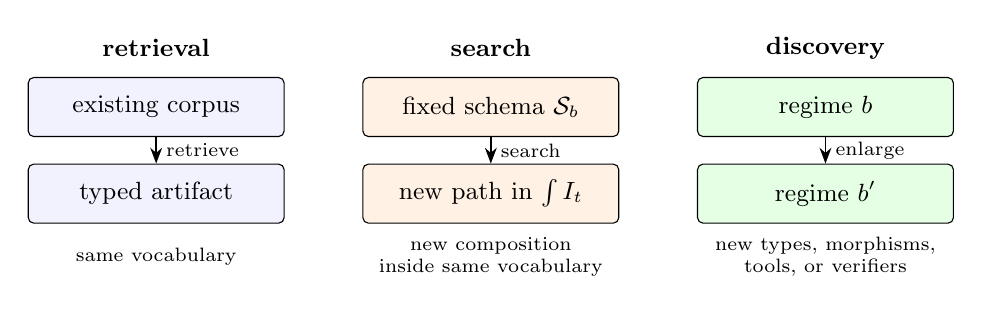
\begin{tikzpicture}[
  box/.style={draw,rounded corners=2pt,fill=blue!5,minimum width=3.25cm,minimum height=0.75cm,align=center,font=\small},
  sbox/.style={draw,rounded corners=2pt,fill=orange!10,minimum width=3.25cm,minimum height=0.75cm,align=center,font=\small},
  dbox/.style={draw,rounded corners=2pt,fill=green!10,minimum width=3.25cm,minimum height=0.75cm,align=center,font=\small},
  arr/.style={-{Stealth[length=2mm]},line width=0.6pt}
]
\node[box] (r1) at (0,0) {existing corpus};
\node[box] (r2) at (0,-1.1) {typed artifact};
\draw[arr] (r1) -- node[right,font=\scriptsize]{retrieve} (r2);
\node[font=\bfseries\small] at (0,0.75) {retrieval};

\node[sbox] (s1) at (4.25,0) {fixed schema $\Sschema_b$};
\node[sbox] (s2) at (4.25,-1.1) {new path in $\int I_t$};
\draw[arr] (s1) -- node[right,font=\scriptsize]{search} (s2);
\node[font=\bfseries\small] at (4.25,0.75) {search};

\node[dbox] (d1) at (8.5,0) {regime $b$};
\node[dbox] (d2) at (8.5,-1.1) {regime $b'$};
\draw[arr] (d1) -- node[right,font=\scriptsize]{enlarge} (d2);
\node[font=\bfseries\small] at (8.5,0.75) {discovery};
\node[font=\scriptsize,align=center] at (0,-1.9) {same vocabulary};
\node[font=\scriptsize,align=center] at (4.25,-1.9) {new composition\\inside same vocabulary};
\node[font=\scriptsize,align=center] at (8.5,-1.9) {new types, morphisms,\\tools, or verifiers};
\end{tikzpicture}
\caption{Retrieval, search, and discovery are structurally different operations. Retrieval adds an already representable artifact. Search finds a new path or object inside a fixed schema. Discovery changes the regime in which artifacts and operations are typed.}
\label{fig:retrieval_search_discovery}
\end{figure}

This view accommodates both compact experimental systems and large distributed systems. In ProtAgents, the schema contains sequences, structures, force predictions, and protein-design hypotheses \citep{ghafarollahi_protagents_2024}. In Sparks and SciAgents, it contains research goals, generated hypotheses, executable plans, code outputs, and reports \citep{ghafarollahi_sparks_2025,ghafarollahi_sciagents_2025}. In ScienceClaw $\times$ Infinite, it contains an extensible skill registry, immutable artifacts with typed metadata and parent lineage, shared open needs, pressure scores, and discourse artifacts exposed to community feedback \citep{wang_scienceclaw_infinite_2026}. The objects differ, but the structural skeleton is the same.

\begin{table}[t]
\centering
\footnotesize
\setlength{\tabcolsep}{4pt}
\begin{tabular}{@{}>{\raggedright\arraybackslash}p{0.22\linewidth}>{\raggedright\arraybackslash}p{0.33\linewidth}>{\raggedright\arraybackslash}p{0.35\linewidth}@{}}
\toprule
Implementation object & Categorical object & Role in discovery system \\
\midrule
artifact type & object of schema category $\Sschema_b$ & declares what kind of thing may be produced \\
tool or skill signature & morphism of $\Sschema_b$ & declares allowed transformation between types \\
current artifact population & copresheaf $I_t:\Sschema_b\to\Set$ & stores artifacts inhabiting each type \\
artifact DAG or hypergraph & category of elements $\int I_t$, or a multicategorical provenance analogue & realized provenance graph \\
accepted update & natural/refinement morphism & preserves prior typed provenance \\
gate or verifier & predicate or scoring functional & decides commitment, rejection, or supersession \\
new schema/tool/verifier & regime extension $u:\Sschema_b\to\Sschema_{b'}$ & changes the admissible scientific vocabulary \\
\bottomrule
\end{tabular}
\caption{Dictionary between implementation terms and the categorical formalism used in this paper.}
\label{tab:dictionary}
\end{table}

\subsection{Artifact states are copresheaves}
\label{sec:copresheaf_results}

The clean mathematical object behind the typed artifact graph is a copresheaf (Definition~\ref{def:copresheaf}). Fix a discovery regime $b$ (Definition~\ref{def:regime}). The regime includes a schema category $\Sschema_b$: its objects are artifact types and its morphisms are allowed operations. A scientific state at time $t$ is a covariant Set-valued functor
\begin{equation}
I_t:\Sschema_b\longrightarrow \Set .
\label{eq:copresheaf_state}
\end{equation}
For each type $A$, the set $I_t(A)$ contains the artifacts of type $A$ currently available to the system. For each operation $f:A\to B$, the function $I_t(f):I_t(A)\to I_t(B)$ records how an artifact of type $A$ gives rise to an artifact of type $B$, when that operation has been realized.

For a materials scientist, typical fibers are:
\[
I_t(\mathrm{PDBChain}),\qquad
I_t(\mathrm{ContactGraph}),\qquad
I_t(\mathrm{SymbolicDAG}),
\]
the current PDB chains, the contact graphs constructed from them, and the candidate or accepted symbolic models. The actual provenance DAG is recovered by the category of elements $\int_{\Sschema_b} I_t$. Its objects are pairs $(A,x)$, where $A$ is a type and $x\in I_t(A)$ is an artifact of that type. A morphism $(A,x)\to(B,y)$ is an operation $f:A\to B$ such that $I_t(f)(x)=y$. Thus the category of elements is not a metaphor for provenance. It is the typed provenance graph.

\begin{figure}[t]
\centering
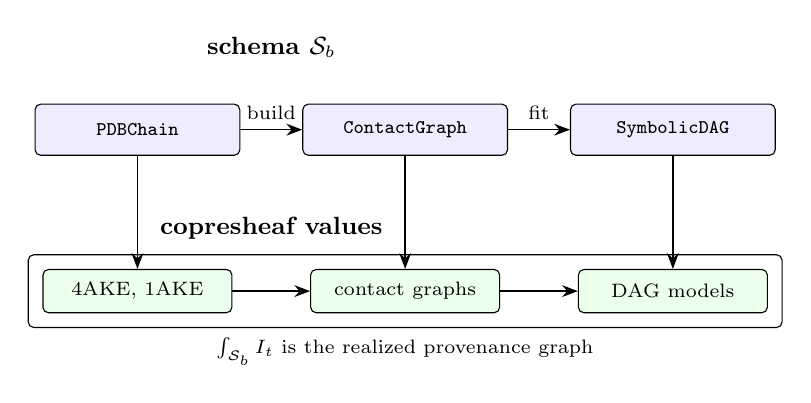
\begin{tikzpicture}[
  type/.style={draw,rounded corners=2pt,fill=blue!7,minimum width=2.6cm,minimum height=0.65cm,align=center,font=\scriptsize},
  art/.style={draw,rounded corners=2pt,fill=green!8,minimum width=2.4cm,minimum height=0.55cm,align=center,font=\scriptsize},
  arr/.style={-{Stealth[length=2mm]},line width=0.55pt}
]
\node[font=\bfseries\small] at (1.7,1.05) {schema $\Sschema_b$};
\node[type] (pdb) at (0,0) {\texttt{PDBChain}};
\node[type] (cg) at (3.4,0) {\texttt{ContactGraph}};
\node[type] (mdl) at (6.8,0) {\texttt{SymbolicDAG}};
\draw[arr] (pdb) -- node[above,font=\scriptsize]{build} (cg);
\draw[arr] (cg) -- node[above,font=\scriptsize]{fit} (mdl);

\node[font=\bfseries\small] at (1.7,-1.25) {copresheaf values};
\node[art] (p1) at (0,-2.05) {4AKE, 1AKE};
\node[art] (c1) at (3.4,-2.05) {contact graphs};
\node[art] (m1) at (6.8,-2.05) {DAG models};
\draw[arr] (pdb) -- (p1);
\draw[arr] (cg) -- (c1);
\draw[arr] (mdl) -- (m1);
\draw[arr] (p1) -- (c1);
\draw[arr] (c1) -- (m1);

\node[draw,rounded corners=2pt,fit=(p1)(m1),inner sep=0.18cm,label={[font=\scriptsize]below:$\int_{\Sschema_b} I_t$ is the realized provenance graph}] {};
\end{tikzpicture}
\caption{A fixed regime has a schema category $\Sschema_b$ of types and operations. A copresheaf $I_t:\Sschema_b\to\Set$ assigns actual artifacts to each type. The category of elements $\int I_t$ is the realized typed artifact DAG.}
\label{fig:copresheaf_elements}
\end{figure}

Copresheaves are the right level of abstraction because they separate a regime from its current contents. The schema can remain fixed while the artifact population grows. Conversely, a discovery move can change the schema while preserving the old artifact population by transport into a new regime. This separation is exactly what is missing when all artifacts, operations, and updates are collapsed into one untyped graph.

\begin{remark}[Yoneda reading]
\label{rem:yoneda}
For a type $A$, the representable copresheaf $\Sschema_b(A,-)$ encodes all operations that can be applied to a generic artifact of type $A$. An actual artifact $x\in I_t(A)$ induces, by the covariant Yoneda lemma, a natural transformation $\Sschema_b(A,-)\to I_t$: each operation out of $A$ is sent to the artifact obtained by applying that operation to $x$. In implementation terms, an artifact is known by the typed operations it can participate in and the downstream artifacts those operations produce.
\end{remark}

\subsection{Fixed-regime updates are endofunctorial under explicit assumptions}
\label{sec:endofunctor_results}

Inside a fixed regime $b$, an agentic system updates artifact states. Write $[\Sschema_b,\Set]$ for the functor category of copresheaves on $\Sschema_b$. Abstractly, a fixed-regime update is an operation on copresheaves,
\begin{equation}
\Phi_b:[\Sschema_b,\Set]\longrightarrow [\Sschema_b,\Set].
\label{eq:fixed_update}
\end{equation}
It reads the current artifact population, selects compatible operations, proposes new artifacts, applies a gate, and returns the next artifact population. The statement that $\Phi_b$ is an endofunctor is a further preservation claim: after the category of admissible refinements between artifact states is specified, $\Phi_b$ must extend from an object-level update to a map on refinement morphisms in the corresponding category of knowledge states $\K_b$ (Definition~\ref{def:fixedupdate}). For the structural observations and the Kan proposition, $\K_b$ is the subcategory of $[\Sschema_b,\Set]$ in which morphisms are componentwise injective natural transformations (Methods, Section~\ref{sec:methods}); refinements may add, annotate, or supersede artifacts, but may not silently identify two previously distinct accepted artifacts.

This qualification matters. A raw program that takes a JSON artifact ledger to another JSON artifact ledger is only an endomap. It becomes an endofunctor only when it also preserves refinement morphisms: if one artifact state extends another by adding verified artifacts without overwriting prior provenance, the updated state should extend the updated predecessor in the same way. This is the formal version of a familiar engineering requirement: if a pipeline is refactored, old valid workflows must still compose.

In code, this is an audit contract rather than a slogan. The implementation must maintain stable artifact identifiers, typed tool or skill signatures, explicit parent lineage, append-only or explicit supersession semantics, status records for failed or retried calls, and no silent merge or deletion of accepted artifacts. When these conditions hold at the committed-state layer, a refinement $\alpha:I\to J$ can be pushed through the update to give a refinement $\Phi_b(\alpha):\Phi_b(I)\to\Phi_b(J)$. When they fail, the system may still be useful, but the endofunctor model applies only after adding the missing audit structure.

Real systems may be stochastic because agents sample, tools fail, schedulers branch, and human feedback arrives asynchronously. Then $\Phi_b$ should be read as a relation, a stochastic kernel, or a morphism in a Kleisli category for an appropriate probability monad \citep{moggi_monads_1991}. This view accommodates sampling-based agents, noisy verifiers, and partial reductions of the artifact graph without changing the structural claims of the framework. The deterministic notation is used because it displays the structural claim clearly; the categorical account is not tied to determinism.

This distinction is important in the examples below. Builder/Breaker is closest to the strict model at the layer of MDL-accepted symbolic DAGs and accumulated evidence, not at the raw proposal trace. ScienceClaw $\times$ Infinite is close at the architecture level because immutable artifacts and parent lineage are already present, but a fully endofunctorial implementation would require checked schema signatures and explicit refinement maps between artifact states.

\subsection{Discovery is regime transition, not only iteration}

\label{sec:regime_enlargement_results}

Search is iteration of $\Phi_b$ inside a fixed regime. Discovery requires a transition to a new regime (Definition~\ref{def:transition}). Let
\begin{equation}
u:\Sschema_b\longrightarrow \Sschema_{b'}
\label{eq:schema_extension}
\end{equation}
be a schema map from the old regime to the new one. In the simplest case, $u$ is an inclusion that preserves old types and operations while adding new ones. In more realistic cases, it may also refine old types, split a type into subtypes, add a verifier, or add new morphisms between old objects. Therefore the general notion should not be restricted to a fully faithful embedding of categories; discovery may add new admissible relations among old objects.

The old artifact state is transported into the new schema by left Kan extension:
\begin{equation}
\Lan_u I_t:\Sschema_{b'}\longrightarrow \Set .
\label{eq:lan_transport}
\end{equation}
For an object $A'$ of the new schema, the value $(\Lan_u I_t)(A')$ is computed as a colimit over the old artifacts that map toward $A'$ (the precise formula appears as Eq.~\ref{eq:lan_formula} in Methods). Operationally, it is the least systematic way to reinterpret old artifacts inside the new vocabulary. If $A'$ receives no morphisms from the image of $u$, the comma category indexing the colimit is empty, so $(\Lan_u I_t)(A')=\varnothing$: free transport supplies nothing at that isolated new type. If $A'$ does receive a morphism from an old type, then old evidence can be transported to it, even if $A'$ itself is a new object. A discovery move is therefore not merely $\Lan_u I_t$; it is transport plus a verified post-transition state containing new evidence, new artifacts, new verifier outcomes, or new grammar productions that are not accounted for by transport alone.

\begin{figure}[t]
\centering
\begin{tikzcd}[row sep=large,column sep=large]
I_t \arrow[r, "\Phi_b"] \arrow[d, "\Lan_u"'] & I_{t+1} \arrow[d, "\Lan_u"] \\
\Lan_u I_t \arrow[r, dashed, "\Lan_u(\Phi_b)"'] & \Lan_u I_{t+1} \arrow[r, "\bar\rho_{t+1}"] & I'_{t+1}
\end{tikzcd}
\caption{Fixed-regime operation is the update $\Phi_b$ inside a schema $\Sschema_b$. The lower dashed arrow is not an independent new-regime dynamics; it is the transported old update $\Lan_u(\Phi_b)$. Thus the left square commutes by functoriality of left Kan extension. Discovery enters through the comparison map $\bar\rho_{t+1}$ from transported evidence to the verified post-transition state (Definition~\ref{def:transition}). In general $\Lan_u I_{t+1}\neq I'_{t+1}$; the comparison map and the residual artifacts outside its image record what the discovery move added beyond functorial transport.}
\label{fig:kan_extension}
\end{figure}

This gives a precise form to the slogan that discovery changes the world model. It does not mean the old world disappears. The old artifacts persist as transported evidence, and their old provenance must remain auditable. What changes is the regime in which the evidence can be represented and composed.

The Kan-extension picture also gives a quantitative reading of how much discovery has occurred, but only after one additional datum is specified. A verified transition includes a natural transformation
\[
\rho:I_t\longrightarrow u^* I'_{t+1},
\]
where $u^*$ restricts a new-regime state back to the old schema. This map says, explicitly, how each old accepted artifact is preserved in the new state. By the adjunction $\Lan_u\dashv u^*$, $\rho$ corresponds uniquely to a comparison map
\[
\bar\rho:\Lan_u I_t\longrightarrow I'_{t+1}.
\]
The image of $\bar\rho$ is the transported-evidence substate. Artifacts outside this image, object by object, are the empirical or representational content the system had to acquire beyond functorial reinterpretation of old evidence. When the new regime carries a relative description-length functional $L_{b'}(-\mid-)$, the \textbf{discovery cost} is the bit budget $L_{b'}(I'_{t+1}\mid\mathrm{im}(\bar\rho))$ required to specify the post-transition state given transported evidence. The Builder/Breaker model in Section~\ref{sec:builder_breaker_results} uses the MDL gate to measure this kind of cost in a concrete protein-mechanics regime.

\subsection{The Builder/Breaker model gives a quantitative MDL case}
\label{sec:builder_breaker_results}

The Builder/Breaker protein-mechanics model is a compact empirical instance of the framework \citep{buehler_break_world_2026} (Definition~\ref{def:bb}\footnote{Code at \url{https://github.com/lamm-mit/BreakingTheWorld}.}). The Breaker chooses new proteins intended to expose failure modes of the current symbolic model. The Builder proposes symbolic DAG edits. The gate accepts a candidate only if it reduces total description length after paired refitting on the same accumulated evidence:
\begin{equation}
L(M,D)=L_{\mathrm{model}}(M)+L_{\mathrm{data}}(D\mid M).
\label{eq:case_mdl_results}
\end{equation}
Here $M$ is the symbolic DAG world model and $D$ is the accumulated protein-mechanics evidence. If the Breaker adds stress-test evidence $E$, a proposed revision $M'$ becomes part of the world model only when
\[
L(M',D\cup E)<L(M,D\cup E),
\]
after both models have been judged on the same evidence. This is the formal sense in which a productive failure becomes scientific structure: the new symbolic law must explain the counterexamples well enough to pay for its additional bits.

The relevant fixed schema contains PDB chains, C$\alpha$ coordinates, contact graphs, Kirchhoff matrices, GNM spectra, compliance observables, slow-mode observables, feature terms, symbolic DAGs, B-factor targets, and MDL budgets. The physical base is the elastic-network and Gaussian Network Model tradition, where low-resolution harmonic contact networks explain slow collective motions and residue-level temperature factors from structure alone \citep{tirion_elastic_1996,bahar_gnm_1997,haliloglu_gaussian_1997}. For a protein chain $p$ with residues $i=1,\ldots,N_p$ and C$\alpha$ coordinates $\mathbf r_{pi}\in\mathbb R^3$, define the contact graph by
\[
A^{(p)}_{ij}
=\mathbf 1\{i\neq j,\ \|\mathbf r_{pi}-\mathbf r_{pj}\|<r_c\},
\qquad r_c=10.0~\text{\AA}.
\]
The GNM Kirchhoff matrix is
\[
\Gamma^{(p)}_{ij}=
\begin{cases}
-A^{(p)}_{ij}, & i\neq j,\\
\sum_{k\neq i} A^{(p)}_{ik}, & i=j .
\end{cases}
\]
Diagonalize
\[
\Gamma_p\mathbf u_{pk}=\lambda_{pk}\mathbf u_{pk},
\qquad
0=\lambda_{p1}\leq\lambda_{p2}\leq\cdots\leq\lambda_{pN_p}.
\]
The all-mode compliance of residue $i$ is the diagonal of the pseudoinverse,
\[
C_{pi}
=(\Gamma_p^+)_{ii}
=\sum_{\lambda_{pk}>0}\frac{u_{pik}^2}{\lambda_{pk}}.
\]
For connected contact graphs this is the familiar sum over $k=2,\ldots,N_p$; the positive-eigenvalue form is the correct pseudoinverse expression if a cutoff or chain segmentation produces additional zero modes.
This is not an arbitrary learned feature. It is the harmonic-network compliance implied by the residue contact topology. In the standard GNM relation,
\[
\langle \Delta R_{pi}^2\rangle
=\frac{3k_B T}{\gamma}\,C_{pi},
\qquad
B_{pi}^{\mathrm{GNM}}
=\frac{8\pi^2}{3}\langle \Delta R_{pi}^2\rangle,
\]
where $\gamma$ is the effective spring constant. Because the learning target is normalized within each chain, the global constants $T$, $\gamma$, and $8\pi^2/3$ drop out. The experimental target is the per-chain normalized C$\alpha$ crystallographic B-factor,
\[
B^{(z)}_{pi}=\frac{B_{pi}-\overline{B}_p}{s_{B,p}},
\]
so the model explains within-chain flexibility patterns rather than absolute crystallographic scale. The physically important caveat is that crystallographic B-factors include thermal motion, static disorder, refinement effects, and crystal-packing effects; the discovery task is therefore to find a compact structural proxy for the experimental pattern, not a complete molecular dynamics law.

Let $z_p(x_i)=(x_i-\overline{x}_p)/s_{x,p}$ denote per-chain normalization. The log-compliance feature and slowest collective-mode participation are
\[
\phi_{pi}=z_p\!\left(\log(C_{pi}+\epsilon)\right),
\qquad
\psi_{pi}=\left[z_p\!\left(|u_{pi2}|\right)+\theta\right]_+ ,
\]
where $[x]_+=\max(x,0)$, $\epsilon>0$ is a small numerical floor inside the logarithm, and $u_{p2}$ denotes the first nonzero GNM eigenmode, called \texttt{mode1\_abs\_z} in the run after taking absolute value and z-scoring. If a contact graph has more than one zero mode, $u_{p2}$ should be read as the first positive-eigenvalue mode. The shift $\theta$ is added before the ReLU, so it acts as a lower clip rather than a conventional threshold; the equivalent threshold form is $[z_p(|u_{pi2}|)-\tau]_+$ with $\tau=-\theta$, and the fitted $\theta=2.2678$ corresponds to clipping near the lowest observed value of $z_p(|u_{pi2}|)$ on the mixed validation slice, so $\psi_{pi}$ shifts first-mode participation onto a positive scale and zeroes only the residues that barely participate in the dominant collective deformation. The discovered symbolic law has the form
\begin{equation}
\boxed{
\widehat B^{(z)}_{pi}
=\alpha+\beta\,\phi_{pi}\psi_{pi}
}
\label{eq:bfactor_symbolic_form}
\end{equation}
or, expanded in the GNM spectrum,
\begin{equation}
\boxed{
\begin{aligned}
\widehat B^{(z)}_{pi}
&=\alpha+\beta\,
z_p\!\left(
\log\!\left(\sum_{\lambda_{pk}>0}\frac{u_{pik}^2}{\lambda_{pk}}+\epsilon\right)
\right)\\
&\quad{}\times
\left[z_p\!\left(|u_{pi2}|\right)+\theta\right]_+ .
\end{aligned}
}
\label{eq:bfactor_spectral_form}
\end{equation}
The fitted numerical values accepted by the MDL gate are $\alpha=-0.1332$, 
$\beta=0.2239$, and $\theta=2.2678$.
The important discovery event is not merely the use of a normal mode; normal modes are available from the start. Categorically, this is not the appearance of an isolated new object. It is the transition at which the schema admits a new multi-input morphism
\[
\texttt{LogNormCompliance}\times \texttt{ReLUModeAmpl}
\longrightarrow
\texttt{ModeConditionedCompliance},
\]
whose target is composite-reachable from old physics-derived quantities only after the new unary transforms and product operation are admitted. The audit below makes this composite reachability explicit. Mechanically, the resulting interaction supports a new explanatory role: local softness matters most when it is expressed along a global collective deformation, rather than acting as an independent additive cause.

For additional context the four outer iterations are summarized in Fig.~\ref{fig:case_dagmdl}. Iteration 0 fits a minimal local fluctuation model on compact proteins. Iteration 1 adds boundary and slow-mode structure for terminal flexibility and gains $9.0$ bits. Iteration 2 exposes a hinge/domain-motion regime, using open and closed adenylate kinase (PDB chains 4AKE and 1AKE) as the canonical conformational stress test, and reorganizes the DAG around collective-motion interpretation at $37.3$ bits gain. Iteration 3 searches inside the enlarged regime on a mixed validation slice and consolidates the model into the compact multiplicative law in Eq.~\ref{eq:bfactor_spectral_form}, at $54.3$ bits gain. The point of the trajectory is not that successive regressions improved monotonically; it is that the admissible symbolic vocabulary was repeatedly stress-tested, revised, and compressed until the surviving law expressed a new mechanics relation.

Equation~\ref{eq:bfactor_spectral_form}, with the numerical values above, is the final accepted symbolic world model for the run. It has a clear mechanical reading. The factor $\phi_{pi}=z_p(\log(C_{pi}+\epsilon))$ is a compressed local-compliance coordinate: it is positive for residues whose contact-network environment predicts above-average fluctuation and negative for mechanically buried or strongly constrained residues. The factor $\psi_{pi}=[z_p(|u_{pi2}|)+2.2678]_+$ is a nonnegative participation weight for the slowest collective mode; the threshold is near the lowest observed value of $z_p(|u_{pi2}|)$ in the mixed validation stage, so the ReLU mostly shifts first-mode participation onto a positive scale and suppresses residues that barely participate in the dominant collective deformation. Their product says that experimental B-factor variation is best compressed by \emph{mode-conditioned compliance}: a residue has high predicted B-factor when it is locally soft in the GNM sense and participates strongly in the dominant collective motion. Local softness that is not aligned with the slow mode is down-weighted, and slow-mode participation without local compliance is insufficient.

The result is not a first-principles derivation from an atomistic Hamiltonian or a crystallographic refinement model, and it is not a neural-network predictor or unconstrained curve fit. The physics sits in the typed compositional pipeline
\[
\{\mathbf r_{pi}\}\longmapsto A_p\longmapsto \Gamma_p
\longmapsto \{(\lambda_{pk},\mathbf u_{pk})\}_{k}
\longmapsto (C_{pi},|u_{pi2}|)
\longmapsto \widehat B^{(z)}_{pi}.
\]
The discovery system searches over symbolic compositions of these physically meaningful artifacts and accepts a revised composition only when it compresses broader evidence better after paying for complexity. Thus the learned law is a mechanics-based constitutive surrogate: not ``B-factor equals an arbitrary fitted expression,'' but
\[
\text{within-chain B-factor pattern}
\sim
\text{all-mode elastic compliance}
\times
\text{slow collective-mode participation}.
\]
The log transform is also physically meaningful because raw GNM fluctuations are heavy-tailed; the model discovered that experimental B-factors are better described by a compressed fluctuation scale than by unbounded raw compliance. The key scientific claim is therefore structural: experimental protein flexibility is not governed by local elastic compliance alone, but by local compliance expressed through participation in the dominant collective mode of the contact-network spectrum.

A post-hoc Kan-transport audit of the run makes the categorical content of this discovery explicit (Fig.~\ref{fig:kan_audit_builder_breaker} and Table~\ref{tab:kan_audit}). The audit constructs a finite schema for each accepted outer iteration, transports the old accumulated artifact state into the next schema, and separates three cases. A new type is \emph{generator-reachable} when it receives an immediate unary generating morphism from an old type. A new type is \emph{composite-reachable} when it is not generator-reachable but becomes reachable through new intermediate types or multi-input operations admitted by the enlarged regime. A type is \emph{isolated} when it is unreachable even by such composites. This distinction matters for the final protein law. The features \texttt{LogNormCompliance} and \texttt{ReLUModeAmpl} are generator-reachable from old physics-derived quantities: they are new transformations of already available compliance and slow-mode amplitude. By contrast, \texttt{ModeConditionedCompliance} is composite-reachable only: it appears when the new regime admits the product operation
\[
\texttt{LogNormCompliance}\times \texttt{ReLUModeAmpl}
\longrightarrow
\texttt{ModeConditionedCompliance}.
\]
Thus the final discovery is not that GNM compliance or the slow collective mode exists; both are already present in the old schema. The new scientific commitment is the interaction type that lets local compliance be conditioned by participation in a collective deformation, and the MDL gate accepts this commitment with a $54.3$-bit gain on the accumulated evidence. The signed model-code changes reinforce the same interpretation: the first accepted transition increases model description length by $39.1$ bits, whereas the later accepted transitions reduce it by $14.4$ and $10.3$ bits. Discovery in this run is therefore not monotone accumulation of terms; it includes retraction and compression of the symbolic vocabulary.

\begin{figure}[t]
\centering
\resizebox{\linewidth}{!}{%
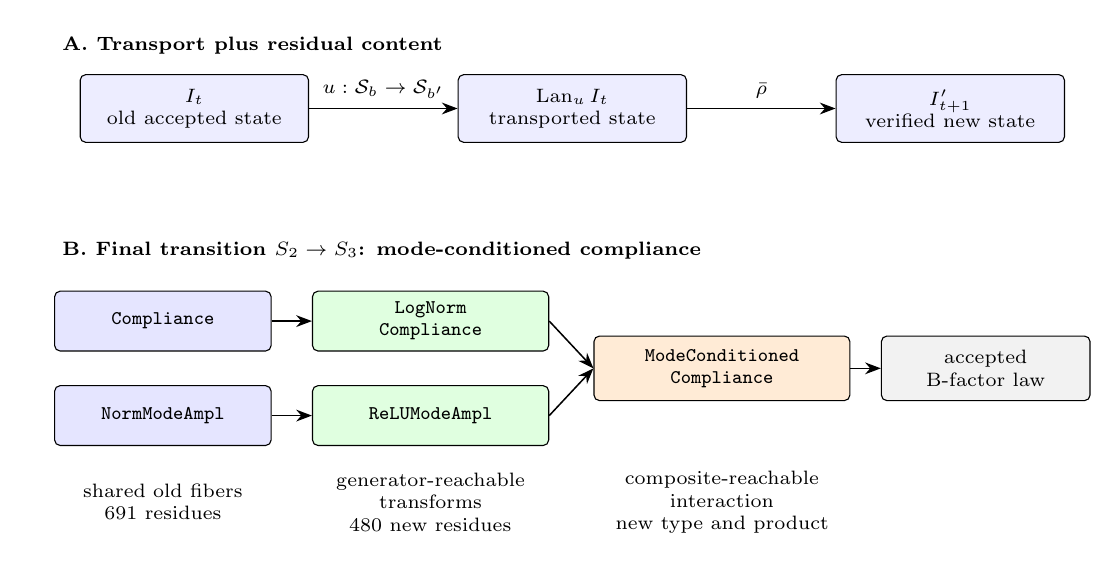
\begin{tikzpicture}[
  font=\scriptsize,
  state/.style={draw,rounded corners=2pt,fill=blue!7,minimum width=2.9cm,minimum height=0.86cm,align=center,font=\scriptsize},
  shared/.style={draw,rounded corners=2pt,fill=blue!10,minimum width=2.75cm,minimum height=0.76cm,align=center,font=\scriptsize},
  unary/.style={draw,rounded corners=2pt,fill=green!12,minimum width=3.0cm,minimum height=0.76cm,align=center,font=\scriptsize},
  comp/.style={draw,rounded corners=2pt,fill=orange!16,minimum width=3.25cm,minimum height=0.82cm,align=center,font=\scriptsize},
  target/.style={draw,rounded corners=2pt,fill=gray!10,minimum width=2.65cm,minimum height=0.82cm,align=center,font=\scriptsize},
  note/.style={font=\scriptsize,align=center,text width=3.2cm},
  arr/.style={-{Stealth[length=2mm]},line width=0.55pt}
]

\node[anchor=west,font=\bfseries\scriptsize] at (-6.6,3.15) {A. Transport plus residual content};
\node[state] (it) at (-4.8,2.35) {$I_t$\\old accepted state};
\node[state] (lan) at (0,2.35) {$\Lan_u I_t$\\transported state};
\node[state] (ip) at (4.8,2.35) {$I'_{t+1}$\\verified new state};
\draw[arr] (it) -- node[above] {$u:\Sschema_b\to\Sschema_{b'}$} (lan);
\draw[arr] (lan) -- node[above] {$\bar\rho$} (ip);

%\draw[black!35] (-6.6,1.05) -- (6.6,1.05);

\node[anchor=west,font=\bfseries\scriptsize] at (-6.6,0.55) {B. Final transition $S_2\to S_3$: mode-conditioned compliance};

\node[shared] (c) at (-5.2,-0.35) {\texttt{Compliance}};
\node[shared] (m) at (-5.2,-1.55) {\texttt{NormModeAmpl}};
\node[unary] (lc) at (-1.8,-0.35) {\texttt{LogNorm}\\\texttt{Compliance}};
\node[unary] (rm) at (-1.8,-1.55) {\texttt{ReLUModeAmpl}};
\node[comp] (mc) at (1.9,-0.95) {\texttt{ModeConditioned}\\\texttt{Compliance}};
\node[target] (bf) at (5.25,-0.95) {accepted\\B-factor law};

\draw[arr] (c) -- (lc);
\draw[arr] (m) -- (rm);
\draw[arr] (lc.east) -- (mc.west);
\draw[arr] (rm.east) -- (mc.west);
\draw[arr] (mc) -- (bf);

\node[note] at (-5.2,-2.65) {shared old fibers\\$691$ residues};
\node[note] at (-1.8,-2.65) {generator-reachable transforms\\$480$ new residues};
\node[note,text width=3.6cm] at (1.9,-2.65) {composite-reachable interaction\\new type and product};

\end{tikzpicture}%
}
\caption{Kan-transport audit of the Builder/Breaker protein-mechanics run. (A) A verified transition transports the old artifact state by $\Lan_u$ and compares it with the accepted new state by $\bar\rho$; residual content records what is added beyond functorial transport. (B) In the final transition, log-compliance and shifted ReLU mode participation are generator-reachable transformations of old physics-derived quantities, whereas \texttt{ModeConditionedCompliance} is reachable only after the new regime admits a product operation. This is the categorical form of the mechanics insight in Eq.~\ref{eq:bfactor_spectral_form}.}
\label{fig:kan_audit_builder_breaker}
\end{figure}

\begin{table}[t]
\centering
\footnotesize
\setlength{\tabcolsep}{3.5pt}
\begin{tabular}{>{\raggedright\arraybackslash}p{0.75cm}
                >{\raggedright\arraybackslash}p{1.4cm}
                >{\raggedright\arraybackslash}p{2.65cm}
                >{\raggedright\arraybackslash}p{2.45cm}
                >{\raggedright\arraybackslash}p{2.1cm}
                >{\raggedright\arraybackslash}p{1.0cm}
                >{\raggedright\arraybackslash}p{1.0cm}}
\toprule
Move & Break type & Generator-reachable new types & Composite-reachable new types & Retracted types & $\Delta L_M$ & MDL gain \\
\midrule
$0\to1$ & regime split & ReLU compliance; terminal exposure & boundary product & old linear parameters & $+39.1$ bits & $+9.0$ bits \\
$1\to2$ & ontology break & none beyond shared GNM base & none beyond shared GNM base & terminal and boundary feature family; old parameters & $-14.4$ bits & $+37.3$ bits \\
$2\to3$ & regime split & log-compliance; ReLU mode amplitude & mode-conditioned compliance & additive-model parameters & $-10.3$ bits & $+54.3$ bits \\
\bottomrule
\end{tabular}
\caption{Two-level Kan audit of the Builder/Breaker transitions. Generator-reachable types receive an immediate unary morphism from old schema objects. Composite-reachable types require new intermediate structure or a newly admitted multi-input composition. Parameter objects are singletons in the audit; they are listed only when they affect the interpretation of a transition. The signed $\Delta L_{\rm model}$ records whether the symbolic model code grew or shrank. MDL gains are acceptance gains from paired refitting on the same accumulated evidence, not a direct numerical discovery cost.}
\label{tab:kan_audit}
\end{table}

\begin{figure}[t]
\centering
\IfFileExists{Fig_101.pdf}{%
    \includegraphics[width=\linewidth]{Fig_101.pdf}%
}{%
    \fbox{\parbox[c][6.5cm][c]{0.95\linewidth}{\centering\textit{[Place \texttt{Fig\_101.pdf} in the same directory as this paper.]}}}%
}
\caption{Builder/Breaker trajectory for residue-level protein mechanics, reproduced from \citep{buehler_break_world_2026}. The trajectory shows symbolic DAG revisions, MDL budget, and fit metrics across staged evidence. The key categorical event is the transition from local flexibility search to a regime that can represent mode-conditioned compliance as an admissible explanatory artifact.}
\label{fig:case_dagmdl}
\end{figure}

The non-monotonic $R^2$ trajectory, $0.48\to0.69\to0.54\to0.41$, is not a failure of the framework. It is the expected signature of a widening evidence set. Discovery is not identified by monotonic fit on heterogeneous data. It is identified by survival of a revised symbolic structure under a stricter compression test on broader evidence. Retractions are central: if a previous feature cannot be transported naturally into the enlarged regime and cannot pay for itself under paired refitting, it must be removed.

The inner symbolic search makes this selectivity visible (Fig.~\ref{fig:case_hillclimb}). Of $144$ proposed DAG edits, only $16$ survive the MDL gate; accepted moves include removals as well as additions. The gate is therefore not decorative. It determines which proposed structures become committed scientific artifacts.

\begin{figure}[t]
\centering
\IfFileExists{Fig_100.pdf}{%
    \includegraphics[width=0.95\linewidth]{Fig_100.pdf}%
}{%
    \fbox{\parbox[c][6cm][c]{0.95\linewidth}{\centering\textit{[Place \texttt{Fig\_100.pdf} in the same directory as this paper.]}}}%
}
\caption{Inner symbolic search in the Builder/Breaker case study, reproduced from \citep{buehler_break_world_2026}. Most proposed DAG edits fail to earn their bits. The accepted sequence contains both additions and retractions, illustrating that a scientific gate must support revision, not only accumulation.}
\label{fig:case_hillclimb}
\end{figure}

\subsection{ScienceClaw $\times$ Infinite gives a distributed architecture case}
\label{sec:scienceclaw_results}

ScienceClaw $\times$ Infinite instantiates the same mathematics at a larger architectural scale \citep{wang_scienceclaw_infinite_2026} (\footnote{Code at \url{https://github.com/lamm-mit/scienceclaw} and \url{https://github.com/lamm-mit/infinite}.}). ScienceClaw supplies the execution substrate: an extensible registry of typed scientific skills, immutable artifacts with metadata and parent lineage, shared open needs, plannerless coordination, pressure scoring, and mutation of the active artifact graph. Infinite supplies the discourse substrate: structured posts, hypotheses, methods, findings, links among claims, votes, comments, reputation, and moderation. Together they make scientific work auditable across both computation and communication.

The implemented structure should be read precisely. Let $A_t$ be the finite set of ScienceClaw artifacts visible at time $t$, and let
\[
\tau:A_t\longrightarrow T
\]
assign each artifact its recorded artifact type. At minimum, this gives a family
\[
I_t(X)=\{a\in A_t:\tau(a)=X\},\qquad X\in T,
\]
that is, a copresheaf over the discrete category of implemented artifact types. Each artifact $a$ also records a skill label $\sigma(a)$, a producer agent, a content hash, and a parent list $p(a)=(a_1,\ldots,a_k)$. Thus the realized computational record is not merely a set of files but a typed acyclic hypergraph whose generating operations have the form
\[
(a_1,\ldots,a_k)\xrightarrow{\ \sigma(a)\ } a .
\]
The unary shadow of this hypergraph generates a free provenance category $\Prov_t$; the full multi-parent synthesis structure is more accurately read as a typed multicategory or colored-operadic provenance record. This is weaker than a software-enforced schema category, and should not be overclaimed. It is nevertheless already enough to support the central categorical interpretation: realized scientific work is a typed population of artifacts together with composable, auditable generating operations.

Open needs add the missing-hole structure. A need signal specifies a desired artifact type, query, rationale, and optional preferred skills. In categorical terms, it marks an unfilled target object or missing cone in the active provenance diagram. The ArtifactReactor does not yet solve a formal Kan-extension or lifting problem; it performs the implemented engineering analogue, using pressure scores and schema overlap to find artifacts and skills that may complete the diagram. Mutation then changes the active subgraph by marking artifacts active, rejected, superseded, or pruned while retaining immutable lineage.

Infinite extends this provenance record into scientific discourse. A post is not just text; it is a typed claim artifact with hypothesis, method, findings, evidence, links, and feedback. Links such as extension, contradiction, replication, or citation are discourse morphisms. Votes, comments, and reputation are verifier signals. The current integration therefore defines an implemented publication map from ScienceClaw artifacts and parent relations into Infinite posts, artifact records, and discourse links. It is not yet a certified functor in software, but it has the functorial shape required for one: computational lineage is carried into a public, inspectable, revisable scientific record.

\begin{figure}[t]
\centering
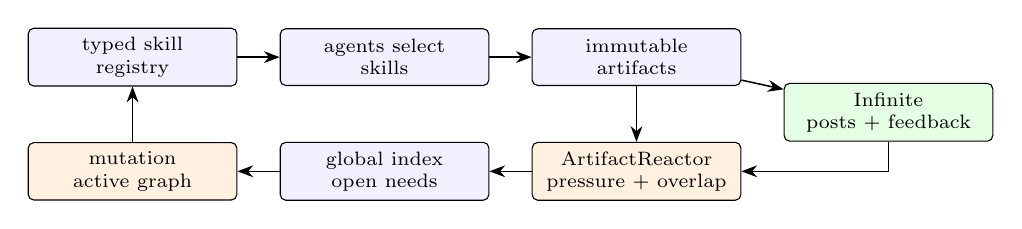
\begin{tikzpicture}[
  box/.style={draw,rounded corners=2pt,fill=blue!6,minimum width=2.65cm,minimum height=0.72cm,align=center,font=\scriptsize},
  gate/.style={draw,rounded corners=2pt,fill=orange!12,minimum width=2.65cm,minimum height=0.72cm,align=center,font=\scriptsize},
  disc/.style={draw,rounded corners=2pt,fill=green!10,minimum width=2.65cm,minimum height=0.72cm,align=center,font=\scriptsize},
  arr/.style={-{Stealth[length=2mm]},line width=0.55pt}
]
\node[box] (skills) at (0,0) {typed skill\\registry};
\node[box] (agents) at (3.2,0) {agents select\\skills};
\node[box] (arts) at (6.4,0) {immutable\\artifacts};
\node[gate] (reactor) at (6.4,-1.45) {ArtifactReactor\\pressure + overlap};
\node[box] (index) at (3.2,-1.45) {global index\\open needs};
\node[gate] (mut) at (0,-1.45) {mutation\\active graph};
\node[disc] (inf) at (9.6,-0.7) {Infinite\\posts + feedback};
\draw[arr] (skills) -- (agents);
\draw[arr] (agents) -- (arts);
\draw[arr] (arts) -- (reactor);
\draw[arr] (reactor) -- (index);
\draw[arr] (index) -- (mut);
\draw[arr] (mut) -- (skills);
\draw[arr] (arts) -- (inf);
\draw[arr] (inf) |- (reactor);
\end{tikzpicture}
\caption{ScienceClaw $\times$ Infinite as a distributed typed artifact system. ScienceClaw executes typed skill compositions and records immutable lineage; the ArtifactReactor and mutation layer coordinate active search; Infinite turns computational artifacts into public scientific discourse with feedback that can re-enter the discovery loop.}
\label{fig:scienceclaw_infinite}
\end{figure}

\paragraph{A concrete instance: SSTR2 peptide design.}
The SSTR2 peptide-design investigation gives a concrete instance of this structure (Fig.~\ref{fig:sstr2_scienceclaw}). The scientific question was whether single-point mutations of a somatostatin-derived peptide could improve predicted binding-related sequence fitness while preserving receptor-binding constraints. The implemented artifact population includes a retrieved SSTR2 peptide-bound structure from PDB 7XNA, contact fingerprints for the receptor--peptide interface, aligned somatostatin-derived peptide sequences, conservation maps, ESM-2 pseudo-log-likelihood mutation scans, physicochemical profiles, ranked candidates, figures, and a synthesized Infinite post. A compressed provenance diagram is
\[
\begin{gathered}
a_{\rm PDB}\xrightarrow{\rm contacts}a_{\rm hotspot},\qquad
a_{\rm seq}\xrightarrow{\rm alignment}a_{\rm cons},\qquad
a_{\rm seq}\xrightarrow{\rm ESM2}a_{\rm PLL},\\
(a_{\rm hotspot},a_{\rm cons},a_{\rm PLL})\xrightarrow{\rm synthesis}a_{\rm claim}.
\end{gathered}
\]
The resulting claim is not that the agents proved binding affinity. Rather, the autonomous analysis found convergent evidence that the K--T--C/CWKTCT-like motif forms a receptor-binding anchor, while surrounding residues define a more permissive mutational region. The same case also illustrates the limit of the current implementation: docking and molecular dynamics were not part of this run, so the Infinite claim remains a structured, provenance-backed hypothesis rather than a validated affinity prediction.

\begin{figure}[t]
\centering
\IfFileExists{Fig_102.pdf}{%
    \includegraphics[width=0.82\linewidth]{Fig_102.pdf}%
}{%
    \fbox{\parbox[c][6cm][c]{0.9\linewidth}{\centering\textit{[Place \texttt{Fig\_102.pdf} in the same directory as this paper.]}}}%
}
\caption{Autonomous agent analyses of the SSTR2 peptide-design landscape, reproduced from \citep{wang_scienceclaw_infinite_2026}. The figure shows a receptor--peptide contact fingerprint and the comparison between conservation and ESM-2 mutation-fitness signals. Categorically, the figure is a terminal visualization artifact generated from a multi-parent provenance cone: structural contacts, sequence alignment, conservation, and language-model scoring are synthesized into a public claim about constrained and mutable regions of the peptide design space.}
\label{fig:sstr2_scienceclaw}
\end{figure}

This case also broadens the notion of a gate. Builder/Breaker uses MDL because the world model is a symbolic equation and the evidence is quantitative. ScienceClaw $\times$ Infinite uses a richer gate: pressure scoring, schema overlap, conflict resolution, status updates, discourse feedback, and reputation. The categorical framework is deliberately agnostic about the scoring functional. What matters is that the gate be typed, auditable, and compatible with provenance.


\FloatBarrier

\subsection{CategoryScienceClaw mechanics as typed discovery graphs}
\label{sec:categoryscienceclaw_mechanics}

CategoryScienceClaw makes the ScienceClaw architecture in Section~\ref{sec:scienceclaw_results} operational at the level of individual scientific claims. In the mechanics runs considered here, the system does not merely store a final plot or a text summary. It records a typed discovery graph whose objects include imported structures, computational surrogates, synthetic computational inputs, formal descriptors, candidate models, rejected alternatives, model gates, stress tests, validation records, figures, and reports. The important point is that these are not only file names. They are typed artifacts connected by morphisms: contact analysis maps a PDB chain to a contact-hotspot descriptor; CSV parsing and regression map force-extension or stress-strain tables to fitted mechanics models; graph scoring maps adhesion/cytoskeleton records to load-path rankings; curvature-energy evaluation maps a membrane field and material model to an energy proxy. The rendered figure is therefore a terminal artifact of a provenance cone, not a decorative illustration appended after the computation.

This mechanics example also clarifies why accepted and rejected models are categorical data. An accepted model is a committed object together with the morphisms that produced it and the gate that certified it. A rejected alternative is not a failure to be deleted; it is an explicit contrast object that records which simpler or weaker explanation did not survive the same evidence. A gate is a typed constraint on a comparison morphism: linear force-extension must outperform a mean-force descriptor, anisotropic orientation-tensor stiffness must explain the network better than an isotropic fiber-count scalar, force-path regression must improve over adhesion alone, and Helfrich-style curvature energy must add material-mechanics content beyond a curvature-only shape descriptor. This is the same logic as the Builder/Breaker MDL case, but here the gate is distributed across mechanics-specific diagnostics rather than one symbolic description-length budget.

The four runs deliberately mix evidence classes. The 7T10 case uses an imported real PDB structure and an imported computational force-extension surrogate. The fiber-network, mechanobiology, and membrane runs use deterministic synthetic computational inputs generated to instantiate the mechanics question when no measured data were present. These synthetic inputs are useful because they test whether the categorical pipeline can generate, route, evaluate, reject, and interpret mechanics hypotheses; they are not biological measurements. Thus the discovery claim is not that new experiments were performed, but that the system can transform a mechanics question into auditable computational evidence and make the accepted/rejected structure explicit.

\begin{table}[t]
\centering
\footnotesize
\setlength{\tabcolsep}{3pt}
\begin{tabular}{@{}>{\raggedright\arraybackslash}p{0.17\linewidth}>{\raggedright\arraybackslash}p{0.22\linewidth}>{\raggedright\arraybackslash}p{0.22\linewidth}>{\raggedright\arraybackslash}p{0.29\linewidth}@{}}
\toprule
Run & Accepted model & Rejected alternative & Mechanics result and categorical role \\
\midrule
7T10 structure-contact mechanics & linear force-extension model with contact-hotspot anchor & mean-force null descriptor & Hotspot positions $[8,9,6,7,1,11]$ define a structural anchoring object; the force-extension morphism gives stiffness $253.1~\mathrm{pN\,nm^{-1}}$, peak force $767.0~\mathrm{pN}$, work $1141.3~\mathrm{pN\,nm}$, and $R^2=0.943$. \\
Fiber-network mechanics & orientation-tensor anisotropic stiffness surrogate & isotropic fiber-count descriptor & A deterministic 12-fiber network yields order parameter $0.673$, principal orientation $47.9^\circ$, stiffness $119.4~\mathrm{kPa}$, and $R^2=0.999989$, turning orientation structure into a typed anisotropic-mechanics object. \\
Mechanobiology force paths & graph-conditioned force-path regression & adhesion-only traction model & A 12-path adhesion/cytoskeleton graph identifies path 12 as the strongest traction-proxy route; adhesion alone gives only moderate fit ($R^2=0.399$), so the accepted morphism includes cytoskeletal coupling, displacement, and path length. \\
Membrane biophysics & Helfrich-style quadratic curvature-energy proxy & curvature-only shape descriptor & A $7\times7$ curvature field with bending modulus $20~k_B T$ gives RMS curvature $0.155~\mathrm{\mu m^{-1}}$ and total energy proxy $11.73~k_B T$, making material energy the accepted target object rather than geometry alone. \\
\bottomrule
\end{tabular}
\caption{CategoryScienceClaw mechanics runs as accepted/rejected categorical evidence. Each row records an accepted model, an explicit rejected alternative, the gate or diagnostic that separates them, and the scientific mechanics content carried by the accepted artifact. Synthetic computational inputs are treated as computational evidence, not as measurements.}
\label{tab:categoryscienceclaw_mechanics_models}
\end{table}

Figure~\ref{fig:csc_7t10_mechanics} shows the most concrete bridge between molecular structure and mechanics. The contact-hotspot object is produced from the 7T10 PDB chain by structure-contact analysis, while the force-extension object is produced from the surrogate force table by CSV parsing and regression. The categorical point is that these two branches meet in a mechanics claim: localized receptor--peptide contacts define plausible load-transfer anchors, and the force-extension gate selects an extension-dependent tensile descriptor over a mean-force null.

\begin{figure}[t]
\centering
\IfFileExists{\CSCMechFigBase/fig1_7t10_discovery_mechanics.pdf}{%
    
\includegraphics[width=\linewidth]{\CSCMechFigBase/fig1_7t10_discovery_mechanics.pdf}%
}{%
    \fbox{\parbox[c][6cm][c]{0.95\linewidth}{\centering\textit{[Missing CategoryScienceClaw figure: fig1\_7t10\_discovery\_mechanics.pdf]}}}%
}
\caption{CategoryScienceClaw 7T10 mechanics figure. The panels combine contact-hotspot concentration, a force-extension trace, and a model gate comparing the accepted linear tensile response with a rejected mean-force descriptor. Categorically, the figure is a terminal visualization artifact generated from a provenance cone containing an imported PDB structure, a force-extension surrogate, a contact-analysis morphism, a regression morphism, and a gate certifying the accepted mechanics claim.}
\label{fig:csc_7t10_mechanics}
\end{figure}

The fiber-network and mechanobiology runs demonstrate two different ways in which graph structure becomes mechanics. In Fig.~\ref{fig:csc_fiber_mechanics}, the relevant new object is an anisotropic stiffness surrogate: the orientation tensor is not merely a descriptive statistic, but a morphism from network geometry to a load-bearing axis and stiffness scale. In Fig.~\ref{fig:csc_mechanobiology_mechanics}, the accepted model is a path-level force-routing object. The rejected adhesion-only alternative is scientifically important because it prevents the system from overinterpreting a single scalar adhesion score as the whole mechanotransduction explanation.

\begin{figure}[t]
\centering
\IfFileExists{\CSCMechFigBase/fig2_fiber_network_discovery_mechanics.pdf}{%
    
\includegraphics[width=\linewidth]{\CSCMechFigBase/fig2_fiber_network_discovery_mechanics.pdf}%
}{%
    \fbox{\parbox[c][6cm][c]{0.95\linewidth}{\centering\textit{[Missing CategoryScienceClaw figure: fig2\_fiber\_network\_discovery\_mechanics.pdf]}}}%
}
\caption{CategoryScienceClaw fiber-network mechanics figure. The figure renders orientation-tensor structure, stress-strain fitting, an accepted anisotropic stiffness surrogate, and a rejected isotropic descriptor. The categorical role of the figure is to expose a typed transition from raw synthetic computational network geometry to a mechanics object whose accepted model commits to anisotropy, not only fiber count.}
\label{fig:csc_fiber_mechanics}
\end{figure}

\begin{figure}[t]
\centering
\IfFileExists{\CSCMechFigBase/fig3_mechanobiology_discovery_mechanics.pdf}{%
    
\includegraphics[width=\linewidth]{\CSCMechFigBase/fig3_mechanobiology_discovery_mechanics.pdf}%
}{%
    \fbox{\parbox[c][6cm][c]{0.95\linewidth}{\centering\textit{[Missing CategoryScienceClaw figure: fig3\_mechanobiology\_discovery\_mechanics.pdf]}}}%
}
\caption{CategoryScienceClaw mechanobiology force-path figure. Load-path ranking, graph visualization, and ablation diagnostics make the accepted force-path regression explicit. Categorically, adhesion, cytoskeletal coupling, displacement, and path length are typed inputs to a multi-parent synthesis morphism whose target is a traction-proxy load-routing claim; the adhesion-only model remains as a rejected contrast object.}
\label{fig:csc_mechanobiology_mechanics}
\end{figure}

The membrane case in Fig.~\ref{fig:csc_membrane_mechanics} is a regime-transition example in miniature. A curvature-only descriptor can represent shape, but the accepted model introduces a material parameter and a quadratic energy functional. The target object is no longer only geometry; it is curvature weighted by bending modulus. This is precisely the kind of enlargement the Kan-obstruction language is meant to identify: old geometric evidence can be transported, but the energy object requires an added morphism and material assumption.

\begin{figure}[t]
\centering
\IfFileExists{\CSCMechFigBase/fig4_membrane_discovery_mechanics.pdf}{%
    
\includegraphics[width=\linewidth]{\CSCMechFigBase/fig4_membrane_discovery_mechanics.pdf}%
}{%
    \fbox{\parbox[c][6cm][c]{0.95\linewidth}{\centering\textit{[Missing CategoryScienceClaw figure: fig4\_membrane\_discovery\_mechanics.pdf]}}}%
}
\caption{CategoryScienceClaw membrane mechanics figure. The curvature heatmap, bending-energy proxy, and modulus sensitivity panels show why the accepted model is a Helfrich-style curvature-energy object rather than a curvature-only shape descriptor. The categorical role is a typed regime enlargement from geometric curvature fields to material energy claims under an explicit validation gate.}
\label{fig:csc_membrane_mechanics}
\end{figure}

Figure~\ref{fig:csc_integrated_mechanics} summarizes the four mechanics runs in the form most relevant to this paper: each panel is organized around a mechanics claim, the computation that supports it, the accepted model, the rejected alternative, and the gate or stress test that separates them. This is why CategoryScienceClaw is more than a plotting layer. It is an implementation of the categorical discovery discipline: scientific results are accepted only as typed, provenance-backed, gate-checked artifacts, while rejected alternatives and limitations remain visible in the graph.

\begin{figure}[t]
\centering
\IfFileExists{\CSCMechFigBase/fig5_integrated_discovery_summary.pdf}{%
    
\includegraphics[width=\linewidth]{\CSCMechFigBase/fig5_integrated_discovery_summary.pdf}%
}{%
    \fbox{\parbox[c][6cm][c]{0.95\linewidth}{\centering\textit{[Missing CategoryScienceClaw figure: fig5\_integrated\_discovery\_summary.pdf]}}}%
}
\caption{Integrated CategoryScienceClaw mechanics summary. The four panels compare molecular contact-supported tensile mechanics, fiber-network anisotropy, graph-mediated mechanobiology force routing, and membrane curvature-energy mechanics. The scientific comparison is inseparable from the categorical one: every panel displays an accepted model, a rejected alternative, and a gate or stress test, making the evidence transformation auditable rather than merely visual.}
\label{fig:csc_integrated_mechanics}
\end{figure}

\FloatBarrier

\subsection{Instantiations across agentic systems}
\label{sec:instantiations}

The same formal pattern appears across several agentic systems developed in this research line, with different regimes, artifact populations, and gates. Table~\ref{tab:systems} summarizes the mapping. The table is deliberately not a leaderboard. It is a structural comparison of how different systems instantiate typed artifact states, fixed-regime updates, and regime-enlarging mechanisms.

\begin{table}[t]
\centering
\footnotesize
\setlength{\tabcolsep}{3pt}
\begin{tabular}{@{}>{\raggedright\arraybackslash}p{0.17\linewidth}>{\raggedright\arraybackslash}p{0.25\linewidth}>{\raggedright\arraybackslash}p{0.25\linewidth}>{\raggedright\arraybackslash}p{0.23\linewidth}@{}}
\toprule
System & Main artifact regime & Gate or verifier & Discovery-relevant mechanism \\
\midrule
ProtAgents \citep{ghafarollahi_protagents_2024} & protein sequences, structures, force and dynamics artifacts & agent critique plus physics and ML tool outputs & physics simulators expose failure modes of generated designs \\
MARS / graph agents & layered material knowledge graphs and substitution candidates & feasibility, manufacturability, and cross-source consistency & cross-layer composition of evidence from heterogeneous corpora \\
Sparks / SciAgents \citep{ghafarollahi_sparks_2025,ghafarollahi_sciagents_2025} & research goals, hypotheses, code, results, and reports & novelty, interestingness, executable results & ideation-to-experiment loops over a research-artifact schema \\
Builder/Breaker \citep{buehler_break_world_2026} & protein-mechanics evidence and symbolic DAG world models & paired MDL compression & adversarial evidence forces retractions and regime enlargement \\
ScienceClaw $\times$ Infinite \citep{wang_scienceclaw_infinite_2026} & typed skills, immutable artifacts, open needs, and discourse artifacts & pressure, schema overlap, mutation, feedback, reputation & plannerless artifact exchange and public claim-level verification \\
\bottomrule
\end{tabular}
\caption{Agentic systems as typed artifact systems. Each system has a schema, artifact population, gate, and mechanism by which the active regime can be stressed or enlarged.}
\label{tab:systems}
\end{table}

\FloatBarrier

\subsection{Relation to existing formalisms}
\label{sec:related}

The problem addressed here also has a historical and philosophical lineage. Bacon and Whewell treated scientific method as an organized practice of collecting, comparing, and conceptually ordering phenomena; Peirce emphasized inquiry as a disciplined process for stabilizing belief under doubt \citep{bacon_novum_organum_1620,whewell_inductive_sciences_1840,peirce_fixation_1877}. Popper, Kuhn, and Lakatos then made failure, anomaly, paradigm change, and research-programme revision central to accounts of scientific progress \citep{popper_logic_1959,kuhn_structure_1962,lakatos_falsification_1970}.

Goethe and Whitehead supply a complementary lineage in which form, relation, and process are primary scientific objects rather than incidental descriptions \citep{goethe_metamorphosis_1790,whitehead_science_modern_world_1925}. Polanyi and Hacking are also relevant: scientific knowledge is not only explicit proposition but skillful practice, and experimental intervention is part of what makes a representation scientifically real \citep{polanyi_personal_knowledge_1958,hacking_representing_intervening_1983}. The contribution of the present paper is to give this broad intuition an auditable mathematical substrate for AI systems: typed artifacts, composable provenance, explicit gates, and verified regime transitions.

The framework is adjacent to, but distinct from, categorical deep learning. Categorical accounts of neural networks and learning, including backpropagation as a functor and categorical deep learning programs based on parametric maps and lenses, clarify the structure of model architectures and training procedures \citep{fong_spivak_tuyeras_2019,gavranovic_cdl_2024,cruttwell_parametric_lenses_2024,crescenzi_zanasi_survey_2024}. The present paper instead studies systems whose state is a typed scientific artifact population and whose most important operation may be a change of regime. The unit of analysis is therefore not only a trained model, but a scientific workflow capable of altering its own schema of admissible artifacts.

The framework also touches coalgebra and dynamical systems. A fixed-regime update resembles a state transition system and can be studied with coalgebraic ideas such as bisimulation and final behavior \citep{aczel_mendler_1989,rutten_coalgebra_2000}. The difference is that discovery changes the state space itself: the relevant trajectory lives over a base of regimes rather than inside one fixed carrier. This is why the indexed or fibered picture is natural.

Finally, the gate connects the framework to MDL, Bayesian model selection, algorithmic information, and open-endedness. MDL and Solomonoff-style compression provide one rigorous account of why a simpler world model that explains broader evidence is preferable \citep{rissanen_mdl_1978,gruenwald_mdl_2007,solomonoff_1964,hutter_aixi_2005,schwarz_bic_1978}. Open-endedness and automated-scientist systems study how systems escape fixed objectives or generate new scientific tasks \citep{stanley_open_endedness_2017,wang_poet_2019,lu_ai_scientist_2024,lu_ai_scientist_v2_2025}. Scientific machine learning supplies many of the typed operators that appear as morphisms in our schemas, from physics-informed learning to operator learning and equation-free multiscale computation \citep{karniadakis_pinns_2021,lu_deeponet_2021,kevrekidis_equation_free_2003}. The contribution here is to place these components into one typed, provenance-preserving, regime-changing account of discovery.

\subsection{Design principles and open problems}
\label{sec:open_results}

The framework suggests five open problems.

\begin{openproblem}[Convergence on growing regimes]
Classical fixed-point theory assumes a fixed underlying space. Discovery systems iterate $\Phi_b$ while also producing regime transitions $b_0\to b_1\to b_2\to\cdots$. Under what conditions does the sequence of transported artifact states converge to a stable object in an appropriate colimit or indexed category? When is non-convergence productive exploration, and when is it unproductive oscillation?
\end{openproblem}

\begin{openproblem}[Scaling laws for discovery]
Standard scaling laws measure loss or benchmark performance inside a fixed regime. Discovery requires a different observable: the rate, quality, and accepted value of regime enlargements. How do discovery rates scale with model size, tool diversity, simulator fidelity, evidence heterogeneity, schema richness, and verifier strength?
\end{openproblem}

\begin{openproblem}[Verification tooling for agentic loops]
The framework requires provenance preservation and gate compatibility. Practical systems need tooling that can replay downstream artifact chains, check approximate naturality, account for description length or pressure scores, and record retractions without deleting provenance.
\end{openproblem}

\begin{openproblem}[Learning the base schema category]
The framework assumes a schema category $\Sschema_b$. Current systems construct it by engineering choice. A major open problem is to learn useful schema categories from corpora, tool signatures, code, figures, equations, and laboratory protocols while keeping morphisms scientifically meaningful. Functorial data migration, olog-style modeling, and category-theoretic accounts of hierarchical materials and building-block replacement provide a starting toolkit \citep{spivak_schemas_2012,buehler_spivak_2011,giesa_spivak_2011_patterns,giesa_spivak_2012_buildingblock}; the open problem is computational: how to learn $\Sschema_b$ and an accompanying description-length functional $L_b$ from data at the scale of working scientific corpora.
\end{openproblem}

\begin{openproblem}[Multicategorical discovery]
The Kan audit in Section~\ref{sec:builder_breaker_results} distinguishes generator-level transport from composite reachability through newly admitted multi-input morphisms. Proposition~\ref{prop:multicat_kan} gives the corresponding multicategorical obstruction under the standard operadic Kan-extension setup. The open problem is now computational and statistical: how can an agentic system learn the typed multicategory or colored-operadic schema $M_b$ from traces, tool signatures, equations, figures, and artifact lineages, and how can it estimate the artifact and operation components of discovery cost at scale?
\end{openproblem}

% =====================================================================
\section{Conclusions and Outlook}
\label{sec:conclusions}
% =====================================================================

This paper has argued that agentic scientific discovery requires two levels of structure. Inside a fixed regime, an agentic system updates typed artifact populations: it adds data, models, simulations, hypotheses, critiques, and reports while preserving provenance. At that level, copresheaves, categories of elements, natural transformations, and endofunctorial dynamics give a precise language for structures already present in working discovery systems. Discovery in the stronger sense occurs when evidence forces a transition to a new regime, and left Kan extension gives the mathematical language for transporting old artifacts into the enlarged vocabulary.

The Builder/Breaker protein-mechanics case shows this structure quantitatively: a symbolic world model is revised by adversarial evidence and an MDL gate, with rejected edits and retractions visible in the audit trail. ScienceClaw $\times$ Infinite shows the same structure architecturally: typed skills, immutable artifacts, open needs, pressure-based coordination, mutation, and public discourse together form a distributed engine for scientific artifact production and revision.

\subsection*{Toward a categorical ScienceClaw $\times$ Infinite}

ScienceClaw $\times$ Infinite is already close to the categorical picture at the level of data model and workflow discipline. It has typed artifact metadata, skill labels, immutable parent lineage, content hashes, open needs, pressure-ranked reactions, mutation of active status, and Infinite posts with hypotheses, methods, findings, artifact records, typed links, votes, comments, and reputation. This is enough to read the current implementation as a typed artifact family equipped with an acyclic provenance hypergraph and a publication map into a discourse graph. What is not yet present is an explicit checked schema category, a certified functor from computation to discourse, or a formal account of schema change.

The next step is therefore not to replace the system, but to lift structures already present in the code into explicit mathematical objects. Skill manifests would become morphism signatures with declared input objects, output objects, constraints, and verifiers. Artifact stores would become materialized fibers of a copresheaf over that schema. Multi-parent synthesis would be treated as a typed multicategory or operadic composition, rather than only as a parent list. Open needs would become typed holes or lifting problems. Infinite would become a discourse category whose objects are claims, posts, artifacts, evidence bundles, objections, replications, and validation signals. The ScienceClaw--to--Infinite integration would then be a checked map from provenance to discourse, preserving identities, parent-child composition, and validation status.

Making this explicit would change the operational status of the platform. The system would no longer merely display provenance; it could verify that provenance diagrams commute, that every public claim has an admissible artifact path, that retractions and supersessions preserve old evidence, and that new artifact types are introduced through recorded schema transitions. In the language of this paper, ScienceClaw $\times$ Infinite would move from a proto-categorical architecture to an executable categorical discovery substrate. The impact would be practical: stronger audit trails, machine-checkable claim lineage, better comparison among autonomous investigations, and a route toward measuring discovery as the residual content added beyond transport of prior evidence.

The central insight is therefore that search is iteration inside a typed scientific regime; discovery is a verified regime transition---enlargement, restructuring, or compression---together with the residual content that lies outside functorial transport of prior evidence.
This statement is mathematical enough to constrain future theory and concrete enough to guide the design of future AI discovery systems.

% =====================================================================
\section{Materials and Methods}
\label{sec:methods}
% =====================================================================

\subsection{Regimes, schemas, and copresheaves}

\begin{definition}[Discovery regime]
\label{def:regime}
A \textbf{discovery regime} is a tuple
\[
b=(\Sschema_b,\Gamma_b,\V_b,L_b),
\]
where $\Sschema_b$ is a small schema category of artifact types and allowed operations, $\Gamma_b$ is a grammar for composing admissible artifacts or model structures, $\V_b$ is a verifier or gate, and $L_b$ is an optional description-length functional. The functional $L_b$ may be presented either absolutely on artifact states or as a relative (conditional) length functional; we write $L_b(I\mid J)$ for the code length of $I$ given a subobject $J\hookrightarrow I$, with $L_b(I)\equiv L_b(I\mid\varnothing)$ recovering the absolute case. In this paper, $\Sschema_b$ carries the main type-and-operation structure; $\Gamma_b$, $\V_b$, and $L_b$ record the additional grammar, acceptance, and scoring data attached to that structure. When these additional data are clear from context, ``regime'' is used informally as shorthand for the schema and its associated commitments.
\end{definition}

\begin{definition}[Artifact-state copresheaf]
\label{def:copresheaf}
For a fixed regime $b$, an \textbf{artifact state at time $t$} is a copresheaf
\[
I_t:\Sschema_b\to\Set .
\]
For each object $A\in\Obj(\Sschema_b)$, $I_t(A)$ is the set of artifacts of type $A$. For each morphism $f:A\to B$, $I_t(f):I_t(A)\to I_t(B)$ maps artifacts along an allowed operation.
\end{definition}

\begin{definition}[Category of elements]
\label{def:elements}
The \textbf{realized provenance category} of $I_t$ is the category of elements $\int_{\Sschema_b}I_t$. Its objects are pairs $(A,x)$ with $x\in I_t(A)$. A morphism $(A,x)\to(B,y)$ is a morphism $f:A\to B$ in $\Sschema_b$ such that $I_t(f)(x)=y$.
\end{definition}

For partially realized scientific workflows, $I_t(f)$ may be a partial function, relation, or span rather than a total function. The total-function presentation is the clean base case; partiality can be handled by replacing $\Set$ with a category of partial maps, relations, spans, or typed records with status events.

\subsection{Fixed-regime update and endofunctoriality}

Let $\K_b$ be a category whose objects are artifact-state copresheaves over $\Sschema_b$ and whose morphisms are provenance-preserving refinements. In the strict presentation used for the structural observations and the Kan proposition, a morphism $\alpha:I_t\to J_t$ is a componentwise injective natural transformation whose components $\alpha_A:I_t(A)\to J_t(A)$ preserve artifact identity, type, and provenance metadata, up to the equivalence or tolerance declared by $\V_b$. The injectivity assumption is the mathematical version of a practical audit rule: a refinement may add, annotate, or supersede artifacts, but it may not silently identify two previously distinct accepted artifacts.

\begin{definition}[Fixed-regime update]
\label{def:fixedupdate}
A \textbf{fixed-regime agentic update} is an endomap on artifact states,
\[
\Phi_b:\Obj(\K_b)\to\Obj(\K_b),
\]
that becomes an endofunctor $\Phi_b:\K_b\to\K_b$ when it maps refinement morphisms to refinement morphisms and preserves identities and composition.
\end{definition}

The update may be implemented by agents, simulators, retrieval systems, symbolic search, or human feedback. The categorical requirement is not that the implementation be deterministic or neural-free, but that the committed state preserve typed provenance. Concretely, an implementation earns the endofunctor notation only when each refinement $\alpha:I\to J$ induces a refinement $\Phi_b(\alpha):\Phi_b(I)\to\Phi_b(J)$ and these induced maps respect identity refinements and composition of refinements. In stochastic or asynchronous implementations, this condition is imposed on the committed-state relation, stochastic kernel, or Kleisli morphism rather than on every raw execution trace.

\subsection{Builder, Breaker, and gates}

\begin{definition}[Builder/Breaker system]
\label{def:bb}
Within a regime $b$, a Builder/Breaker system consists of a proposal mechanism $B$, an evidence-producing mechanism $K$, and a gate $\V_b$. The Breaker $K$ selects or generates evidence intended to stress the current artifact state. The Builder $B$ proposes candidate increments or revisions. The gate $\V_b$ decides whether the candidate is committed, rejected, superseded, or held for review.
\end{definition}

For the protein-mechanics case, the gate is MDL:
\begin{equation}
\V_b(M',M;D)=1
\quad\Longleftrightarrow\quad
L_{\mathrm{model}}(M')+L_{\mathrm{data}}(D\mid M')
<
L_{\mathrm{model}}(M)+L_{\mathrm{data}}(D\mid M).
\label{eq:mdl_methods}
\end{equation}
Comparisons are paired: both models are refit on the same accumulated data $D$. For ScienceClaw $\times$ Infinite, $\V_b$ is pressure-based and social-technical: schema overlap, artifact status, conflict resolution, open-need satisfaction, discourse feedback, and reputation all contribute to commitment.

\subsection{Verified regime transition and Kan transport}

\begin{definition}[Verified regime transition]
\label{def:transition}
Given an old state $I_t\in\K_b$ and a new accepted state $I'_{t+1}\in\K_{b'}$, a \textbf{verified regime transition} from $b$ to $b'$ relative to $(I_t,I'_{t+1})$ consists of a schema functor
\[
u:\Sschema_b\to\Sschema_{b'}
\]
together with a preservation natural transformation
\[
\rho:I_t\longrightarrow u^*I'_{t+1},
\]
where $u^*:[\Sschema_{b'},\Set]\to[\Sschema_b,\Set]$ is restriction along $u$. The state-dependence is part of the data: a verified transition is a piece of structure attached to a specific pair of states, not a universal property of the schemas alone. The transition satisfies three compatibility conditions:
\begin{enumerate}[leftmargin=1.7em,topsep=2pt,itemsep=2pt]
    \item $u$ is faithful on morphisms and injective on objects, except where the transition explicitly records a type split, quotient, or recoding;
    \item $\rho$ is componentwise injective and provenance-preserving, so old accepted artifacts remain inspectable after the transition;
    \item old commitments remain accepted after transport: for predicate-valued gates, $\V_b(I_t)=1$ implies $\V_{b'}(\mathrm{im}(\bar\rho))=1$, where $\bar\rho:\Lan_uI_t\to I'_{t+1}$ is the adjoint transpose of $\rho$.
\end{enumerate}
If a description-length functional is present, the transported old state has no larger code length than the original old state, $L_{b'}(\mathrm{im}(\bar\rho))\le L_b(I_t)$, or else the increase is recorded as an explicit recoding cost. The transition is \textbf{nontrivial} when $\Sschema_{b'}$ contains a new object, morphism, verifier, grammar production, or tool class not generated inside $u(\Sschema_b)$, or when $I'_{t+1}$ contains accepted artifacts not in $\mathrm{im}(\bar\rho)$.
\end{definition}

The transported old artifact state is the left Kan extension
\begin{equation}
(\Lan_u I_t)(A') \cong \colim_{(uA\to A')\in(u\downarrow A')} I_t(A),
\label{eq:lan_formula}
\end{equation}
where the colimit exists because $\Set$ is cocomplete and $\Sschema_b$ is small. If $u$ is fully faithful, the unit $I_t\to u^*\Lan_u I_t$ is an isomorphism, so old fibers are preserved by transport alone. If $u$ is only faithful, if it recodes old object names, or if the new schema adds morphisms among old types, preservation is not automatic; it is supplied by the explicit map $\rho$ in Definition~\ref{def:transition}. When the comma category $(u\downarrow A')$ is empty---that is, when $A'$ receives no morphisms from $u(\Sschema_b)$---the colimit is the initial object of $\Set$, giving $(\Lan_u I_t)(A')=\varnothing$. New evidence then populates such fibers, or activates new morphisms absent from the old regime.

\subsection{Structural observations and the Kan obstruction}

The first three statements are closure and verification observations: they unpack what is already forced by a fixed schema, provenance-preserving refinement, and a declared gate. The first nontrivial categorical obstruction is the Kan statement that follows, where the comparison map makes residual content unavoidable. The later propositions record the functorial consequences needed for auditability, composition of transitions, and the multicategorical reading of product-like discovery moves.

\begin{observation}[Fixed-regime reachability]
\label{obs:reachability}
Let $b$ be fixed and let $\Phi_b:\K_b\to\K_b$ be an endofunctor on artifact states over $\Sschema_b$. For any state $I_0$ and any $n\in\N$, every object appearing in the provenance category $\int \Phi_b^n(I_0)$ lies over an object of $\Sschema_b$. Thus finite iteration of a fixed-regime update cannot by itself create an artifact of a type outside $\Sschema_b$.
\end{observation}

\begin{proof}
Each state in $\K_b$ is by definition a copresheaf on $\Sschema_b$. Applying $\Phi_b$ returns another object of $\K_b$, hence another copresheaf on the same schema. The category of elements of any such copresheaf has objects $(A,x)$ with $A\in\Obj(\Sschema_b)$. Induction on $n$ gives the claim.
\end{proof}

\begin{observation}[Verification requires provenance preservation and a gate]
\label{obs:verification}
Let $\alpha:I\to J$ be a committed update inside a fixed regime $b$. If the update is verified in the sense of the regime, then (i) $\alpha$ preserves prior provenance up to the equivalence or tolerance declared by $\V_b$, and (ii) $\alpha$ passes the gate $\V_b$. Conversely, if both conditions hold and $\V_b$ is the regime's declared acceptance criterion, then the update is verified.
\end{observation}

\begin{proof}
If provenance preservation fails, then at least one previously accepted artifact chain cannot be re-expressed after the update, so the update is not verified. If the gate fails, the update violates the regime's declared commitment criterion. Conversely, provenance preservation keeps old accepted diagrams valid, and the gate supplies the regime-specific acceptance judgment.
\end{proof}

\begin{observation}[Nontrivial discovery requires regime-extending structure]
\label{obs:external}
Let $b$ be fixed. A nontrivial discovery move that produces an artifact over a type, morphism, verifier, grammar production, or tool class absent from $\Sschema_b$ cannot be obtained by finite iteration of $\Phi_b:\K_b\to\K_b$ alone. It requires a verified regime transition $u:\Sschema_b\to\Sschema_{b'}$ or an equivalent schema-generating mechanism.
\end{observation}

\begin{proof}
By Observation~\ref{obs:reachability}, finite iteration of $\Phi_b$ yields artifact states over $\Sschema_b$. Hence it cannot create an artifact whose type is not an object of $\Sschema_b$. Moreover, because $b=(\Sschema_b,\Gamma_b,\V_b,L_b)$ is fixed during iteration, the grammar, verifier, and available tool classes are fixed as well. A move requiring a new type, morphism, verifier, grammar production, or tool class therefore cannot be the result of iteration inside $\K_b$ alone; it requires a transition to a regime in which the new structure exists.
\end{proof}

\begin{proposition}[Kan obstruction to transport-only discovery]
\label{prop:kan_obstruction}
Let $u:\Sschema_b\to\Sschema_{b'}$ and $\rho:I_t\to u^*I'_{t+1}$ be a verified regime transition (Definition~\ref{def:transition}). Let
\[
\bar\rho:\Lan_u I_t\longrightarrow I'_{t+1}
\]
be the unique adjoint transpose of $\rho$ under $\Lan_u\dashv u^*$. Three statements follow.
\begin{enumerate}[leftmargin=1.7em,topsep=2pt,itemsep=2pt]
    \item If $(u\downarrow A')=\varnothing$, then transport is empty at $A'$:
    \[
    (\Lan_u I_t)(A')=\varnothing .
    \]
    If $I'_{t+1}(A')\neq\varnothing$, then $\mathrm{im}(\bar\rho_{A'})=\varnothing$ and the residual at $A'$ is forced to be nonempty. Every artifact accepted at such an $A'$ must be supplied from outside transport of the old regime.
    \item The image $\mathrm{im}(\bar\rho)\subseteq I'_{t+1}$ is a sub-copresheaf of transported evidence. At each object $A'$, the pointwise residual set
    \[
    \mathcal{R}(A') = I'_{t+1}(A') \,\setminus\, \mathrm{im}(\bar\rho_{A'})
    \]
    records artifacts at that type not obtained by functorial transport of old evidence. The categorical object is the inclusion $\mathrm{im}(\bar\rho)\hookrightarrow I'_{t+1}$; the complements $\mathcal{R}(A')$ are an objectwise engineering diagnostic and need not themselves form a sub-copresheaf.
    \item When a relative description-length functional $L_{b'}(-\mid-)$ is present, the \textbf{discovery cost} of the move is
    \[
    L_{b'}\big(I'_{t+1}\mid \mathrm{im}(\bar\rho)\big),
    \]
    the code length of the post-transition state given transported evidence. If $L_{b'}$ is additive on such inclusions, this can be written as $L_{b'}(I'_{t+1})-L_{b'}(\mathrm{im}(\bar\rho))$. In particular, any description-length functional assigning positive conditional length to nonempty forced residuals gives a strictly positive local discovery cost at such a type.
\end{enumerate}
\end{proposition}

\begin{proof}
The adjunction $\Lan_u\dashv u^*$ gives a natural bijection
\[
\mathrm{Nat}(\Lan_u I_t,I'_{t+1})\cong \mathrm{Nat}(I_t,u^*I'_{t+1}),
\]
so $\rho$ determines the unique map $\bar\rho$. Statement~(i) is the pointwise formula~(\ref{eq:lan_formula}) for an empty index category: a colimit over the empty diagram in $\Set$ is the initial object $\varnothing$. Hence the component of $\bar\rho$ at $A'$ has empty domain and empty image, so any accepted element of $I'_{t+1}(A')$ lies outside transport. For (ii), the pointwise image of a natural transformation between Set-valued functors is a subfunctor: naturality sends elements in $\mathrm{im}(\bar\rho_{A'})$ to elements in $\mathrm{im}(\bar\rho_{B'})$ along every morphism $A'\to B'$. Therefore $\mathrm{im}(\bar\rho)$ is the transported-evidence substate, and the pointwise complement records artifacts not in that transported image. Statement~(iii) is the definition of the relative description-length functional on the inclusion $\mathrm{im}(\bar\rho)\hookrightarrow I'_{t+1}$, with strict positivity following from the stated positivity assumption on forced residuals.
\end{proof}

\begin{proposition}[Refinements lift to realized provenance]
\label{prop:elements_functoriality}
Let $b$ be fixed and let $\alpha:I\to J$ be a refinement morphism in $\K_b$, represented in the strict presentation by a componentwise injective natural transformation. Then $\alpha$ induces a faithful functor
\[
\int\alpha:\int_{\Sschema_b} I\longrightarrow \int_{\Sschema_b} J
\]
defined by $(A,x)\mapsto (A,\alpha_A(x))$ on objects and by sending a realized operation $f:(A,x)\to(B,y)$ to the same schema morphism $f:(A,\alpha_A(x))\to(B,\alpha_B(y))$. The assignment $\alpha\mapsto\int\alpha$ preserves identities and composition of refinements.
\end{proposition}

\begin{proof}
If $f:(A,x)\to(B,y)$ is a morphism in $\int_{\Sschema_b}I$, then $I(f)(x)=y$. Naturality of $\alpha$ gives
\[
J(f)(\alpha_A(x))=\alpha_B(I(f)(x))=\alpha_B(y),
\]
so the same schema morphism $f$ is a morphism in $\int_{\Sschema_b}J$. Thus $\int\alpha$ is a functor. It is faithful because it does not change the underlying schema morphism on any hom-set. Identity refinements act as identity functors, and for refinements $\alpha:I\to J$ and $\beta:J\to L$, the componentwise equality $(\beta\circ\alpha)_A=\beta_A\circ\alpha_A$ gives $\int(\beta\circ\alpha)=\int\beta\circ\int\alpha$.
\end{proof}

\begin{remark}
Proposition~\ref{prop:elements_functoriality} is the formal audit rule behind the artifact-ledger language. If a refinement adds, annotates, or supersedes artifacts without identifying previously distinct accepted artifacts, then the realized provenance graph of the predecessor embeds faithfully into the realized provenance graph of the successor. Older lineage queries remain meaningful after accepted refinements.
\end{remark}

\begin{proposition}[Verified regime transitions compose]
\label{prop:transition_composition}
Let $(u,\rho)$ be a verified regime transition from $b$ to $b'$ relative to $(I_t,I'_{t+1})$, and let $(v,\sigma)$ be a verified regime transition from $b'$ to $b''$ relative to $(I'_{t+1},I''_{t+2})$. Assume that gates are hereditary on declared transported substates: whenever a transported state is accepted, any transported substate selected by a preservation map is also accepted. Then
\[
(v\circ u,\tau),\qquad
\tau=(u^*\sigma)\circ\rho:I_t\longrightarrow (v\circ u)^*I''_{t+2},
\]
is a verified regime transition from $b$ to $b''$ relative to $(I_t,I''_{t+2})$. Moreover, under the canonical isomorphism $\Lan_{v\circ u}\cong \Lan_v\Lan_u$, the comparison map $\bar\tau$ factors as
\[
\Lan_{v\circ u}I_t \cong \Lan_v\Lan_u I_t
\xrightarrow{\Lan_v(\bar\rho)}
\Lan_v I'_{t+1}
\xrightarrow{\bar\sigma}
I''_{t+2}.
\]
\end{proposition}

\begin{proof}
The composite $v\circ u$ preserves morphism faithfulness and object injectivity except at type splits, quotients, or recodings explicitly recorded by the two transitions. Since restriction along a composite satisfies $(v\circ u)^*=u^*v^*$, the map $\tau=(u^*\sigma)\circ\rho$ is natural, componentwise injective, and provenance-preserving because both factors are. If $\V_b(I_t)=1$, the first transition accepts the transported image in $b'$. The second transition is relative to the accepted state $I'_{t+1}$ and accepts its transported image in $b''$; heredity on transported substates then gives acceptance of the smaller image of $\bar\tau$. The factorization of $\bar\tau$ follows from uniqueness of left adjoints to restriction: $\Lan_{v\circ u}$ and $\Lan_v\Lan_u$ are both left adjoint to $u^*v^*$, and the displayed composite is the adjoint transpose of $\tau$.
\end{proof}

\begin{remark}
This proposition justifies reading a multi-stage investigation as one audited discovery move when every intermediate transition records a preservation map and clears its gate. In the Builder/Breaker case, the four accepted outer iterations can therefore be viewed both locally, transition by transition, and globally, as a composite map transporting the initial evidence into the final symbolic regime while accumulating residual content.
\end{remark}

\begin{proposition}[Declared old evidence remains inspectable]
\label{prop:evidence_conservativity}
Let $(u,\rho)$ be a verified regime transition from $b$ to $b'$ relative to $(I_t,I'_{t+1})$. For every old type $A$ and artifact $x\in I_t(A)$, the component $\rho_A$ gives a unique preserved artifact $\rho_A(x)\in I'_{t+1}(uA)$ with the same declared identity and provenance metadata, up to the equivalence or tolerance specified by the transition. If $J\hookrightarrow I_t$ is an old accepted evidence substate and the gate-compatibility condition declares its transported image accepted in $b'$, then all artifacts of $J$ remain accepted as transported evidence in $I'_{t+1}$.
\end{proposition}

\begin{proof}
Componentwise injectivity and provenance preservation of $\rho$ are part of Definition~\ref{def:transition}. Therefore distinct old artifacts remain distinct after applying $\rho$, and their recorded lineage remains inspectable in the new state. For an accepted evidence substate $J\hookrightarrow I_t$, restricting $\rho$ gives a preservation map from $J$ into $u^*I'_{t+1}$, equivalently a comparison map from its transported image into $I'_{t+1}$. The gate-compatibility hypothesis then says precisely that this transported image is accepted in $b'$.
\end{proof}

\begin{remark}
The proposition is deliberately about preserved evidence, not about every old model commitment. Discovery systems may explicitly retract, compress, or supersede symbolic model terms when the new gate rejects them on accumulated evidence. What is prohibited is silent deletion of the old evidential record. In the Builder/Breaker audit, the additive-model parameters retracted at the $2\to3$ transition are model commitments recorded as superseded; the protein evidence and its provenance remain available for the accepted multiplicative law.
\end{remark}

\begin{proposition}[Multicategorical Kan obstruction]
\label{prop:multicat_kan}
Assume a regime is presented by a small typed multicategory, or equivalently a colored-operadic schema, whose multimorphisms
\[
\phi:(A_1,\ldots,A_k)\longrightarrow B
\]
declare admissible multi-input scientific operations. Assume artifact states are Set-valued algebras on these schemas and that restriction along a multifunctor $u:M_b\to M_{b'}$ admits a left adjoint $\Lan^{\mathrm m}_u$ computed by the usual operadic comma-colimit construction \citep{leinster_higher_operads_2004}. For a verified multicategorical transition with preservation map $\rho:I_t\to u^*I'_{t+1}$ and adjoint comparison map
\[
\bar\rho:\Lan^{\mathrm m}_u I_t\longrightarrow I'_{t+1},
\]
the following hold.
\begin{enumerate}[leftmargin=1.7em,topsep=2pt,itemsep=2pt]
    \item If the operadic comma category of operations from transported old types into a new type $B$ is empty in every arity, then $(\Lan^{\mathrm m}_u I_t)(B)=\varnothing$. Any accepted artifact at $B$ is forced residual content, exactly as in Proposition~\ref{prop:kan_obstruction}.
    \item If $B$ has no unary generating morphism from the old image but receives a new $k$-ary multimorphism from transported or generator-reachable inputs, then $B$ is not isolated in the multicategorical regime. Its transported part is generated by formal composites of transported input artifacts through that multimorphism, while the newly admitted multimorphism itself is residual schema content.
    \item If the description-length functional separates artifact content from operation-registry content, then the relative discovery cost splits into an artifact residual term and an operation residual term; without additivity, the same statement holds as a subadditive upper bound.
\end{enumerate}
\end{proposition}

\begin{proof}
The proof is the multicategorical analogue of Proposition~\ref{prop:kan_obstruction}. By assumption, $\Lan^{\mathrm m}_u$ is left adjoint to restriction and is computed pointwise by a colimit over the operadic comma category whose objects are multimorphisms from tuples of transported old types to the target type. If this indexing category is empty in every arity, the colimit in $\Set$ is $\varnothing$, forcing any accepted element of $I'_{t+1}(B)$ to lie outside transport. If a $k$-ary multimorphism into $B$ exists, the same comma-colimit has nonempty indexing data in arity $k$ and therefore contains the formal composites obtained by applying that operation to transported input artifacts; applying $\bar\rho$ evaluates those formal composites in the verified new state. Finally, a relative code that is additive over artifact fibers and operation-registry entries gives the stated decomposition of residual cost, while subadditivity gives the upper bound in the nonadditive case.
\end{proof}

\begin{remark}
For the Builder/Breaker $2\to3$ transition, the ordinary generator-level audit sees no unary morphism from the old schema into \texttt{ModeConditionedCompliance}. The multicategorical view sees the binary operation
\[
\texttt{LogNormCompliance}\times\texttt{ReLUModeAmpl}
\longrightarrow \texttt{ModeConditionedCompliance},
\]
whose inputs are themselves generator-reachable transforms of old physics-derived quantities. Thus Table~\ref{tab:kan_audit} and Fig.~\ref{fig:kan_audit_builder_breaker} are the unary-shadow audit of a native multicategorical statement: the target feature is composite-reachable, and the product operation is residual schema content.
\end{remark}


\subsection{CategoryScienceClaw mechanics figure-generation details}
\label{sec:categoryscienceclaw_methods}

The CategoryScienceClaw mechanics case study was generated from the four-run \texttt{formal\_mechanics\_runs} export tree. Each run contains an investigation JSON file, a discovery report, a categorical discovery graph, and, when needed, deterministic computational inputs. The top-level synthesis records the four mechanics claims; the figure agent writes figure results, legends, a manifest, and the PDF figures included in Section~\ref{sec:categoryscienceclaw_mechanics}.

The visualized computations use ScienceClaw skills and deterministic local analyses: structure-contact analysis for 7T10 contact hotspots, CSV parsing and regression for force-extension and stress-strain tables, graph-conditioned load-path scoring for the mechanobiology run, and a Helfrich-style quadratic curvature-energy proxy for the membrane run. Evidence origin is retained in the investigation JSON. The 7T10 structure is imported structural evidence and the force-extension table is an imported computational surrogate. The fiber-network, mechanobiology, and membrane inputs are deterministic synthetic computational inputs, generated because measured fields were not present in the run. The reports therefore treat them as computational surrogates for testing mechanics reasoning and categorical provenance, not as biological measurements.

The categorical discovery graph records candidate models, accepted and rejected status, gates, stress tests, and report/figure artifacts. Thus a plotted panel is traceable back to input artifacts and morphisms rather than being a standalone graphics product. The manuscript figures use the generated PDF outputs directly, preserving the provenance reported by CategoryScienceClaw.

\subsection{Case-study implementation details}

The Builder/Breaker protein-mechanics case uses Gaussian Network Model features derived from PDB chains, symbolic DAG search over physically interpretable factors, and paired MDL comparisons. The Breaker selects staged protein evidence intended to expose failure modes; the Builder proposes edits such as adding factors, removing factors, swapping terms, and thresholding. The existing figures in this manuscript summarize the outer four-stage trajectory and the inner hill-climb search.

The Kan-transport audit in Fig.~\ref{fig:kan_audit_builder_breaker} and Table~\ref{tab:kan_audit} was computed from the accepted world-model records of the same run. For each outer iteration $t$, a finite schema $\Sschema_t$ was constructed whose objects are the typed physics artifacts, observables, symbolic intermediate features, B-factor target, and singleton parameter objects present in the accepted model. The artifact-state fiber size for residue-level objects was taken from the accumulated evidence count recorded in the run, giving $122$, $263$, $691$, and $1171$ residues at iterations $0$ through $3$; chain-level physics objects used the corresponding accumulated chain counts. For each transition $\Sschema_t\to\Sschema_{t+1}$, shared objects were transported by identity. New objects were classified in two passes. First, the generator-level comma diagnostic recorded whether the new object received an immediate unary generating morphism from a shared old object. Second, a composite-reachability pass took the transitive closure through all new morphisms, including multi-input product morphisms. Thus an object such as \texttt{ModeConditionedCompliance} is not generator-reachable from the old schema, but it is composite-reachable through newly admitted morphisms
\[
\texttt{Compliance}\to\texttt{LogNormCompliance},\qquad
\texttt{NormModeAmpl}\to\texttt{ReLUModeAmpl},
\]
followed by the product operation defining \texttt{ModeConditionedCompliance}. This two-level audit avoids treating the empty generator-level comma category as a claim of absolute isolation in the full free category. The residual fiber counts in the audit should therefore be read objectwise: for shared and generator-reachable residue-level types, the $480$-residue residual in the final transition is the newly revealed evidence slice; for composite-reachable types, the essential residual is the new operation and feature type that make the old evidence composable in a new way. MDL break gains are reported as paired acceptance gains, not as the relative code length $L_{b'}(I'_{t+1}\mid\mathrm{im}(\bar\rho))$ itself.

ScienceClaw $\times$ Infinite is treated as an architecture case rather than a numeric MDL case. The implementation provides a skill registry, controlled artifact-type metadata, an evolving artifact ledger, parent-linked immutable lineage, open needs, pressure-based reactions, mutation of active status, and Infinite discourse artifacts with community verifier signals. The formal reading used in the paper is therefore conservative: the code realizes a typed artifact family and an acyclic provenance hypergraph, whose path-category shadow gives the category-of-elements-style structure discussed in the Results. A fully explicit schema category or certified functor from computation to discourse is a natural future implementation, not an assumption about the present code.

% =====================================================================
\section*{Acknowledgments}
% =====================================================================

Support from MGAIC, ONR, ARO, AFOSR, NIH, DSO, NSF, and additional sources is gratefully acknowledged. Part of this work was supported by the U.S. Department of Energy, Office of Science, Office of Advanced Scientific Computing Research and Office of Basic Energy Sciences, Scientific Discovery through Advanced Computing (SciDAC) program under the FORUM-AI project.

% =====================================================================
\section*{Code and Data Availability}
% =====================================================================

Code, generated artifacts, logs, and figures for the Builder/Breaker protein-mechanics case are available at \url{https://github.com/lamm-mit/BreakingTheWorld}. The ScienceClaw framework is available at \url{https://github.com/lamm-mit/scienceclaw}. The Infinite discourse platform is available at \url{https://github.com/lamm-mit/infinite}. 

% =====================================================================
% Bibliography
% =====================================================================

\bibliographystyle{unsrtnat}
\bibliography{refs}

\end{document}
